\documentclass%
%[handout]
{beamer}
% % % % % % % %
% % % % % % % %
% % % % % % % %
%IMPORTANT
%compiles with
%pdflatex -shell-escape
%IMPORTANT
% % % % % % % %
% % % % % % % %
% % % % % % % %
\mode<presentation>
{
\useinnertheme{rounded}
\useoutertheme{infolines}
\usecolortheme{orchid}
\usecolortheme{whale}
}

\usepackage[english]{babel}
\usepackage[latin1]{inputenc}
\usepackage[all,cmtip]{xy}
\usepackage{times}
\usepackage[T1]{fontenc}
\usepackage{ifthen}
\usepackage{amsmath}
\usepackage{amssymb}
\usepackage{cancel}
\usepackage{comment}
\usepackage{multirow}
\usepackage{psfrag}
\usepackage{rotating}
\usepackage{fp}
\usepackage{calc}
\usepackage{bm}
\usepackage[all,cmtip]{xy}
\RequirePackage{xstring}

%%%%%%%%%%%%%%%%%%%%%%%%%%%%%%%%%%%%%%%%%%
%
% List of commands in this document
%
%
% \logdiffbaseandexp
% \logdifftwouponedown
% \productrulefofx
% \quotientruley
% \limitradical  (broken)
% \limitsub
% \chainruley
% \chainrulefofx
% \chainruleStyleOne
% \chainruleStyleTwo
% \chainruleStyleThree
% \infinitelimit
% \limitfactor
% \newtonsmethod
% \constantmultiple
% \chainruletwice
% \youWillNotBeTested
% \optionalDisplay  %Dummy command needed for compatibility with Calculus notes.
% \Arcsin
% \Arccos
% \Arctan
% \Arccot
% \diff
%%%%%%%%%%%%%%%%%%%%%%%%%%%%%%%%%%%%%%%%%%

\newcommand{\diff}{{\normalfont \text{d}}}
\newtheorem{question}{Question}
\newtheorem{observation}{Observation}
\newtheorem{proposition}{Proposition}
\newtheorem{remark}{Remark}
\newcommand{\youWillNotBeTested}{\begin{frame}You will not be tested on the material in the following slide.\end{frame}}
\DeclareMathOperator{\Vol}{Vol}

\DeclareMathOperator{\Arcsin}{\sin^{-1}}
\DeclareMathOperator{\Arccos}{\cos^{-1}}
\DeclareMathOperator{\Arctan}{\tan^{-1}}
\DeclareMathOperator{\Arccot}{{\cot^{-1}}}
\DeclareMathOperator{\Arcsec}{{\sec^{-1}}}
\DeclareMathOperator{\Arccsc}{{\csc^{-1}}}
\DeclareMathOperator{\maclaurin}{{\normalfont{Mc}}}
\newcommand{\taylor}{{\normalfont{T}}}

\newcommand{\optionalDisplay}[1]{#1}
\renewcommand{\Im}{\mathrm{Im}}
\renewcommand{\Re}{\mathrm{Re}}

%\DeclareMathOperator{\Re}{Re}
%\DeclareMathOperator{\Im}{Im}
\newcommand{\fcv}[1]{{\bf #1}} %this command stands for freecalc Vector
\DeclareMathOperator{\curl}{\fcv{curl}}
\DeclareMathOperator{\divg}{div}
\DeclareMathOperator{\proj}{\fcv{proj}}
\DeclareMathOperator{\orth}{\fcv{orth}}
\DeclareMathOperator{\grad}{\fcv{grad}}
\newcommand{\RR}{{\mathbb{R}}}
\newcommand{\cR}{{\mathcal{R}}}
\newcommand{\cD}{{\mathcal{D}}}
\newcommand{\cP}{{\mathcal{P}}}
\newcommand{\fcUncoverAlert}[2]{\uncover<#1->{\alert<#1>{#2}}}
\newcommand{\alertNoH}[2]{\alert<handout:0|#1>{#2}}
\newcommand{\fcAnswerNoH}[2]{
\FPeval{\fcResult}{clip(#1-1)}
\uncover<handout:0|\fcResult>{\alert<handout:0|\fcResult>{\textbf{?} }} \uncover<handout:0| #1->{\alert<handout:0|#1>{\!\!\!#2}}
}
\newcommand{\fcAnswer}[2]{
\FPeval{\fcResult}{clip(#1-1)}
\uncover<handout:0|\fcResult>{\alertNoH{\fcResult}{\textbf{?} }} \uncover<#1->{\alertNoH{#1}{\!\!\!#2}}
}
\newcommand{\fcAnswerUncover}[3]{
\FPeval{\fcResult}{clip(#2-1)}
\uncover<handout:0|#1-\fcResult>{\alertNoH{\fcResult}{\textbf{?}}} \uncover<#2->{\alertNoH{#2}{\!\!\!#3}}
}
\newcommand{\fcAnswerUncoverNoH}[3]{
\FPeval{\fcResult}{clip(#2-1)}
\uncover<handout:0|#1-\fcResult>{\alertNoH{\fcResult}{\textbf{?}}} \uncover<handout:0|#2->{\alertNoH{#2}{\!\!\!#3}}
}

\newcommand{\fcQuestion}[2]{%
\FPeval{\fcResult}{clip(#1+1)}%
\uncover<#1->{\alertNoH{ #1,\fcResult}{#2}}%
}
\newcommand{\fcEvalToInt}[1]{\FPeval{\fcResult}{clip(#1)}\fcResult}
\newcommand{\refBad}[3]{%
\ifthenelse{\equal{#1}{??}}%
{#2}%
{#3}%
}%example usage: \refBad{\ref{eqMacLaurinDef}}{their definition}{their definition (Definition \ref{eqMacLaurinDef})}
\newcommand{\fcCancel}[2]{
\FPeval{\fcResult}{clip(#1-1)}
\only<handout:0|-\fcResult>{#2} \only<#1->{\alertNoH{#1}{\cancel{\alertNoH{0}{#2}}}}
\vphantom{\cancel{#2}}
}
%<-WARNING: the superflous-looking \alertNoH{0} is needed:
% for some unknown to me reason it causes LaTeX to add the correct amount of spacing.

%code blocks regular expression that replaces all strings of the form \alert<handout:0| a> by \alertNoH{a}:
%Find:
%\\alert<[^|^0]*0|\([^>]*\)>
%Replace:
%\\alertNoH{\1}
%code blocks regular expression that replaces all strings of the form \alert<a> but not containing | by \alertNoH{a}:
%Find:
%\\alert<\([^|^>]*\)>
%Replace:
%\\alertNoH{\1}


\newcommand{\fcLicense}{
\begin{frame}
\frametitle{License to use and redistribute}
These lecture slides and their $\LaTeX${} source code are licensed to you under the Creative Commons license CC BY 3.0. You are free
\begin{itemize}
\item to Share - to copy, distribute and transmit the work,
\item to Remix - to adapt, change, etc., the work,
\item to make commercial use of the work,
\end{itemize}
as long as you reasonably acknowledge the original project (a notice of use freecalc is sufficient).
\begin{itemize}
\item Latest version of the .tex sources of the slides: \url{https://sourceforge.net/p/freecalculus/code/HEAD/tree/}
\item Should the link be outdated/moved, search for  ``freecalc project''.
\item Creative Commons license CC BY 3.0:
\url{https://creativecommons.org/licenses/by/3.0/us/}
and the links therein.
\end{itemize}
\end{frame}
}


\newcommand{\onlyNoH}[2]{\only<handout:0|#1>{#2}}
%
%  An example of logarithmic differentiation of a function with a
%  variable base and exponent.
%  #1 is the base.
%  #2 is the exponent.
%  #3 is the derivative of the natural logarithm of the base.
%  #4 is the derivative of the exponent.
%  #5 is (base)(exponent)' + (exponent)(base)' after simplification.
%
\newcommand{\logdiffbaseandexp}[5]{
\begin{example}[Variable base and exponent]
\abovedisplayskip=0pt
\belowdisplayskip=0pt
\abovedisplayshortskip=0pt
\belowdisplayshortskip=0pt
\begin{align*}
\text{Differentiate}\quad \alertNoH{ 13}{y} %
 & \alertNoH{ 13}{=} %
\alertNoH{ 13}{%
#1^{#2}%
}.%
\uncover<2->{%
\intertext{
Take logarithms of both sides:%
}
}%
\uncover<2->{%
\ln y
}%
 & \uncover<2->{ = } %
\uncover<2->{%
\ln #1^{\alertNoH{ 3}{#2}}%
}\\%
\uncover<3->{%
\alertNoH{ 4-5}{\ln y}%
}%
 & \uncover<3->{ = } %
\uncover<3->{%
\alertNoH{ 6-7}{%
\alertNoH{ 3}{#2} \ln #1%
}.}%
\uncover<4->{%
\intertext{
Differentiate implicitly with respect to $x$:%
}%
}%
\fcAnswer{5}{\frac{1}{y} y'}%
 & \uncover<4->{ = } %
\fcAnswerUncover{4}{7}{%
\left( #2 \right) \alertNoH{ 8-9}{\frac{\diff}{\diff x} \left( \ln #1 \right)} + \left( \ln #1 \right)\alertNoH{ 10-11}{\frac{\diff}{\diff x}\left( #2 \right)} %
}\\%
\uncover<8->{%
\frac{1}{\alertNoH{12}{y}} y'%
}%
 & \uncover<8->{ = } %
\uncover<8->{%
( #2 ) \alertNoH{8-9}{\left( \fcAnswerUncover{8}{9}{ #3 }\right)} + \left( \ln #1 \right) \alertNoH{ 10-11}{ \left( \fcAnswerUncover{8}{11}{ #4 } \right) }
}\\%
\uncover<12->{%
y'%
}%
 & \uncover<12->{ = } %
\uncover<12->{%
\alertNoH{ 12-13}{y} \left( #5 \right)%
}\\%
 & \uncover<13->{ = } %
\uncover<13->{%
\alertNoH{ 13}{#1^{#2}} \left( #5 \right).%
}%
\end{align*}
\end{example}
}


%
%  An example of logarithmic differentiation of a function.
%  It looks as follows:
%
%  Differentiate y = (#1 #2)/#3.
%  Take logarithms of both sides:
%  ln y = ln((#1 #2)/#3)
%  ln y = ln#1 + ln#2 - ln#3
%  ln y = #4 + #5 - #6
%  Differentiate implicitly with respect to x:
%  (1/y)y' = #7 + #8 - #9
%  y' = y(#7 + #8 - #9)
%  y' = ((#1 #2)/#3)(#7 + #8 - #9)
%
\newcommand{\logdifftwouponedown}[9]{
\begin{example}[Logarithmic Differentiation%
]
\abovedisplayskip=0pt
\belowdisplayskip=0pt
\abovedisplayshortskip=0pt
\belowdisplayshortskip=0pt
\begin{align*}
\text{Differentiate}\quad \alertNoH{ 18}{y} %
 & \alertNoH{ 18}{=} %
\alertNoH{ 18}{%
\frac{#1 #2}{#3}%
}.%
\uncover<2->{%
\intertext{
Take logarithms of both sides:%
}
}%
\uncover<2->{%
\ln y
}%
 & \uncover<2->{ = } %
\uncover<2->{%
\ln \frac{\alertNoH{ 3-4}{#1}\alertNoH{ 5-6}{#2}}{\alertNoH{ 7-8}{#3}}%
}\\%
\uncover<2->{%
\ln y
}%
 & \uncover<2->{ = } %
\uncover<2->{%
\ln \alertNoH{ 3-4}{#1} + \ln \alertNoH{ 5-6}{#2} -  \ln \alertNoH{ 7-8}{#3}%
}\\%
\uncover<3->{%
\alertNoH{ 9-10}{\ln y}%
}%
 & \uncover<3->{ = } %
\uncover<3->{%
\alertNoH{ 3-4,11-12}{%
\left( \uncover<4->{#4}\right) %
}%
\alertNoH{ 5-6}{%
\uncover<6->{+} \alertNoH{ 13-14}{\left( \uncover<6->{#5}\right)} %
}%
\alertNoH{ 7-8}{%
\uncover<8->{-} \alertNoH{ 15-16}{\left( \uncover<8->{#6}\right)} %
}%
}%
\uncover<9->{%
\intertext{
Differentiate implicitly with respect to $x$:%
}%
}%
\uncover<10->{%
\alertNoH{ 10}{\frac{1}{\alertNoH{ 17}{y}} y'}%
}%
 & \uncover<9->{ = } %
\uncover<9->{%
\alertNoH{ 11-12}{\left( \uncover<12->{#7} \right)} + %
\alertNoH{ 13-14}{\left( \uncover<14->{#8} \right)} - %
\alertNoH{ 15-16}{\left( \uncover<16->{#9} \right)} %
}\\%
\uncover<17->{%
y'%
}%
 & \uncover<17->{ = } %
\uncover<17->{%
\alertNoH{ 17-18}{y} \left( #7 + #8 - #9 \right)%
}\\%
 & \uncover<18->{ = } %
\uncover<18->{%
\alertNoH{ 18}{\frac{#1 #2}{#3}} \left( #7 + #8 - #9 \right)%
}%
\end{align*}
\end{example}
}


%
%  An example of a derivative with the Product Rule, using the symbol f(x).
%  It looks as follows:
%
%  Differentiate f(x) = #1 #2.
%  Product Rule: f'(x) = (#1)(d/dx)(#2) + (#2)(d/dx)(#1)
%   = (#1)(#4) + (#2)(#3)
%   = #5.
%
%  #6 appears in the subtitle of the example.
%
\newcommand{\productrulefofx}[6]{%
\begin{example}[Product Rule%
\ifthenelse{\equal{#6}{0}}%
{}%
{, #6}%
]%
\abovedisplayskip=0pt
\belowdisplayskip=0pt
\abovedisplayshortskip=0pt
\belowdisplayshortskip=0pt
\begin{align*}
\text{Differentiate}\quad f(x) & = \alertNoH{2}{ #1}\alertNoH{3}{ #2.}\\%
\uncover<2->{%
\text{Product Rule:}\quad f'(x)%
}%
& \uncover<2->{%
 =  \alertNoH{ 6-7}{\frac{\diff}{\diff x}\left( \alertNoH{2}{#1} \right)}\left( \alertNoH{3}{#2} \right)+\left( \alertNoH{2}{#1} \right) \alertNoH{ 4-5}{\frac{\diff}{\diff x}\left( \alertNoH{3}{#2} \right)} %
}\\%
& \uncover<4->{%
 = \alertNoH{ 6-7}{\left( \fcAnswerUncover{4}{7}{#3} \right)}\left( #2 \right)+ \left( #1 \right) \alertNoH{ 4-5}{\left(\fcAnswer{5}{ #4 }\right)}  %
}\\%
& \uncover<8->{%
 = #5.%
}%
\end{align*}
\end{example}
}


%
%  An example of a derivative with the Constant Multiple Rule.
%  It looks as follows:
%
%  Find the derivative of #1 = #2.
%   #1 = (#3)(#4).
%   d#1/dx = (d/dx)((#3)(#4))
% Constant Multiple Rule: = (#3)(d/dx)(#4)
%   = (#3)(#5)
%   = #6.
%
%  #7 appears in the subtitle of the example.
%
\newcommand{\constantmultiple}[7]{%
\begin{example}[Constant Multiple Rule%
\ifthenelse{\equal{#7}{0}}%
{}%
{, #7}%
]%
\abovedisplayskip=0pt
\belowdisplayskip=0pt
\abovedisplayshortskip=0pt
\belowdisplayshortskip=0pt
\begin{align*}
\text{Find the derivative of}\quad #1 & = #2.\\%
\uncover<2->{%
#1 %
}%
& \uncover<2->{%
 = \left( #3\right)\left( #4\right).
}\\%
\uncover<3->{%
\frac{\diff #1}{\diff x} %
}%
& \uncover<3->{%
 = \frac{\diff}{\diff x}\left[ \alertNoH{ 4}{\left( #3\right)}\left( #4\right)\right]
}\\%
\uncover<4->{%
\text{Constant Multiple Rule:}\quad %
}%
& \uncover<4->{%
 =  \alertNoH{ 4}{\left( #3\right)}\alertNoH{ 5-6}{\frac{\diff}{\diff x}\left( #4\right)}
}\\%
& \uncover<5->{%
 =  \left( #3\right)\alertNoH{ 5-6}{\left( \fcAnswer{6}{#5}\right)}
}\\%
& \uncover<7->{%
 =  #6.
}%
\end{align*}
\end{example}
}


%
%  An example of a derivative with the Quotient Rule, using the symbol y.
%  It looks as follows:
%
%  Differentiate y = #1 / #2.
%  Quotient Rule: dy/dx = ((#2)(d/dx)(#1)-(#1)(d/dx)(#2))/(#2)^2
%   = ((#2)(#3)-(#1)(#4))/(#2)^2
%   = #5
%   = #6.
%
%  #7 appears in the subtitle of the example.
%
\newcommand{\quotientruley}[7]{%
\begin{example}[Quotient Rule%
\ifthenelse{\equal{#7}{0}}%
{}%
{, #7}%
]%
\abovedisplayskip=0pt
\belowdisplayskip=0pt
\abovedisplayshortskip=0pt
\belowdisplayshortskip=0pt
\begin{align*}
\text{Differentiate}\quad y & = \frac{\alertNoH{2}{ #1}}{\alertNoH{3}{#2}}.%
\uncover<2->{%
\intertext{Quotient Rule:}%
}%
%&\\%
\uncover<2->{%
\frac{\diff y}{\diff x}%
}%
& \uncover<2->{%
 = \frac%
{ \alertNoH{ 4-5}{\frac{\diff}{\diff x}\left( \alertNoH{2}{ #1} \right)}\left( \alertNoH{3}{#2} \right) - \left( \alertNoH{2}{#1} \right) \alertNoH{ 6-7}{\frac{\diff}{\diff x}\left( \alertNoH{3}{#2} \right)}}%
{\left( \alertNoH{3}{#2}\right)^2}%
}\\%
& \uncover<4->{%
 = \frac%
{\alertNoH{ 4-5}{\left(\fcAnswer{5}{ #3 }\right)}\left( #2 \right)  - \left( #1 \right) \alertNoH{ 6-7}{\left( \fcAnswerUncover{4}{7}{#4} \right)}}%
{\left( #2\right)^2}%
}\\%
& \uncover<8->{%
 = #5%
}\\%
& \uncover<9->{%
 = #6.%
}%
\end{align*}
\end{example}
}

%
%  An example of an indefinite integral with the Substitution Rule.
%  It looks as follows:
%
%  Find \int (#1, with nothing substituted for UU and VV).
%  Let u = #2
%  Then du = #3.
%  Therefore #4 = #5.
%  Substitute: \int (#1, with the alert command for u and du
%          substituted for UU and VV respectively)
%  = \int (#6, with the alert command for u and du substituted for UU and VV)
%  = (#7, with u substituted for UU) + C
%  = (#8, with #2 substituted for UU) + C
%
%  #9 appears in the subtitle of the example.
%
\newcommand{\subrule}[9]{%
\begin{example}[Substitution Rule%
\ifthenelse{\equal{#9}{0}}%
{}%
{, #9}%
]%
\abovedisplayskip=0pt
\belowdisplayskip=0pt
\abovedisplayshortskip=0pt
\belowdisplayshortskip=0pt
\begin{align*}
\text{Find}\quad \int %
 \noexpandarg\exploregroups\StrSubstitute{\StrSubstitute{#1}{UU}{3}}{VV}{6-7}\noexploregroups\expandarg. & \\%
\uncover<2->{%
\text{Let}\quad\alertNoH{ 2-3,8,13}{u}%
}%
& \uncover<2->{%
\alertNoH{ 2-3,8,13}{ = \uncover<3->{#2.}}%
}\\%
\uncover<4->{%
\text{Then}\quad \alertNoH{ 4-5}{\diff u}%
}%
& \uncover<4->{%
\alertNoH{ 4-5}{ = \uncover<5->{#3}}%
}\\%
\uncover<6->{%
\alertNoH{ 6-7,9}{#4}%
}%
& \uncover<6->{%
\alertNoH{ 6-7,9}{ = \uncover<7->{#5.}}%
}\\%
\uncover<8->{%
\text{Substitute:}\quad \int%
 \noexpandarg\exploregroups\StrSubstitute{\StrSubstitute{#1}{UU}{8}}{VV}{9}\noexploregroups\expandarg}%
& \uncover<8->{= \alertNoH{ 10-11}{\int\noexpandarg\exploregroups\StrSubstitute{\StrSubstitute{#6}{UU}{8}}{VV}{9}\noexploregroups\expandarg %
}}\\%
& \uncover<10->{\alertNoH{ 10-11}{%
 = \uncover<11->{\noexpandarg\exploregroups \StrSubstitute{#7}{UU}{\alertNoH{ 13}{u}}\noexploregroups\expandarg} \uncover<12->{\alertNoH{ 12}{+C}}%
}}\\%
& \uncover<13->{%
 = \noexpandarg\exploregroups \StrSubstitute{#8}{UU}{\alertNoH{ 13}{#2}}\noexploregroups\expandarg +C.%
}%
\end{align*}
\end{example}
}

%
%  An example of a definite integral with the Substitution Rule.
%  There are nine arguments to the function.  The ninth is a string of four
%  groups of the form {AA}{BB}{CC}{DD} where AA is the lower limit of
%  integration, BB is the upper limit of integration, CC is the lower limit
%  of integration with respect to u, and DD is the upper limit of integration
%  with respect to u.
%  It looks as follows:
%
%  Find \int_{AA}^{BB} (#1, with nothing substituted for UU and VV).
%  Let u = #2
%  Then du = #3.
%  #4 = #5.
%  When x = AA, u = CC.
%  When x = BB, u = DD.
%  Substitute: \int_{AA}^{BB} (#1, with the alert command for u and du
%          substituted for UU and VV respectively)
%  = \int_{CC}^{DD} (#6, with the alert command for u and du substituted for UU and VV)
%  = [#7, with u substituted for UU]_{CC}^{DD}
%  = #8.
%
%
\newcommand{\subruledefbounds}[9]{%
\begin{example}[Substitution Rule, Definite Integral%
]%
\abovedisplayskip=0pt
\belowdisplayskip=0pt
\abovedisplayshortskip=0pt
\belowdisplayshortskip=0pt
\begin{align*}
\text{Find}\quad \int%
_{\StrMid{#9}{1}{1}}%
^{\StrMid{#9}{2}{2}} %
 \noexpandarg\exploregroups\StrSubstitute{\StrSubstitute{#1}{UU}{3}}{VV}{6-7}\noexploregroups\expandarg. & \\%
\uncover<2->{%
\text{Let}\quad\alertNoH{ 2-3,8-12}{u}%
}%
& \uncover<2->{%
\alertNoH{ 2-3,8-12}{ = \uncover<3->{#2.}}%
}\\%
\uncover<4->{%
\text{Then}\quad \alertNoH{ 4-5}{\diff u}%
}%
& \uncover<4->{%
\alertNoH{ 4-5}{ = \uncover<5->{#3}}%
}\\%
\uncover<6->{%
\alertNoH{ 6-7,13}{#4}%
}%
& \uncover<6->{%
\alertNoH{ 6-7,13}{ = \uncover<7->{#5.}}%
}\\%
\uncover<8->{%
\alertNoH{ 8-9,14}{\text{When } x = \StrMid{#9}{1}{1}, \quad u }%
}%
& \uncover<8->{%
\alertNoH{ 8-9,14}{ = \uncover<9->{\StrMid{#9}{3}{3}.}}%
}\\%
\uncover<10->{%
\alertNoH{ 10-11,15}{\text{When } x = \StrMid{#9}{2}{2}, \quad u }%
}%
& \uncover<10->{%
\alertNoH{ 10-11,15}{ = \uncover<11->{\StrMid{#9}{4}{4}.}}%
}\\%
\uncover<12->{%
\text{Substitute:}\quad \int%
_{\alertNoH{ 14}{\StrMid{#9}{1}{1}}}%
^{\alertNoH{ 15}{\StrMid{#9}{2}{2}}} %
 \noexpandarg\exploregroups\StrSubstitute{\StrSubstitute{#1}{UU}{12}}{VV}{13}\noexploregroups\expandarg}%
& \uncover<12->{= \alertNoH{ 16-17}{{\int}%
_{\uncover<14->{\alertNoH{ 14}{
\StrMid{#9}{3}{3}}}}%
^{\uncover<15->{
\alertNoH{ 15}{
\StrMid{#9}{4}{4}}}} %
\noexpandarg\exploregroups\StrSubstitute{\StrSubstitute{#6}{UU}{12}}{VV}{13}\noexploregroups\expandarg %
}}\\%
& \uncover<16->{\alertNoH{ 16-17}{%
 = {\left[ \uncover<17->{%
\noexpandarg\exploregroups\StrSubstitute{#7}{UU}{u}\noexploregroups\expandarg %
}\right]}_{\StrMid{#9}{3}{3}}^{\StrMid{#9}{4}{4}}%
}}\\%
& \uncover<18->{%
 = #8.
}%
\end{align*}
\end{example}
}


%
%  An example of a definite integral with the Substitution Rule.
%  There are nine arguments to the function.  The ninth is a string of two
%  groups of the form {AA}{BB} where AA is the lower limit of
%  integration and BB is the upper limit of integration.
%  It looks as follows:
%
%  Find \int_{AA}^{BB} (#1, with nothing substituted for UU and VV).
%  Let u = #2
%  Then du = #3.
%  #4 = #5.
%  Substitute: \int (#1, with the alert command for u and du
%          substituted for UU and VV respectively)
%  = \int (#6, with the alert command for u and du substituted for UU and VV)
%  = #7, with u substituted for UU
%  = #8.
%  Therefore int_{AA}^{BB} (#1, with nothing substituted for UU and VV)
%      = [#8]_{AA}^{BB}
%  = #9.
%
%
\newcommand{\subruledefvar}[9]{%
\begin{example}[Substitution Rule, Definite Integral%
]%
\abovedisplayskip=0pt
\belowdisplayskip=0pt
\abovedisplayshortskip=0pt
\belowdisplayshortskip=0pt
\begin{align*}
\text{Find}\quad \int%
_{\StrMid{#9}{1}{1}}%
^{\StrMid{#9}{2}{2}} %
 \noexpandarg\exploregroups\StrSubstitute{\StrSubstitute{#1}{UU}{3}}{VV}{6-7}\noexploregroups\expandarg. & \\%
\uncover<2->{%
\text{Let}\quad\alertNoH{ 2-3,8,12}{u}%
}%
& \uncover<2->{%
\alertNoH{ 2-3,8,12}{ = \uncover<3->{#2.}}%
}\\%
\uncover<4->{%
\text{Then}\quad \alertNoH{ 4-5}{\diff u}%
}%
& \uncover<4->{%
\alertNoH{ 4-5}{ = \uncover<5->{#3}}%
}\\%
\uncover<6->{%
\alertNoH{ 6-7,9}{#4}%
}%
& \uncover<6->{%
\alertNoH{ 6-7,9}{ = \uncover<7->{#5.}}%
}\\%
\uncover<8->{%
\text{Substitute:}\quad \int%
 \noexpandarg\exploregroups\StrSubstitute{\StrSubstitute{#1}{UU}{8}}{VV}{9}\noexploregroups\expandarg}%
& \uncover<8->{= \alertNoH{ 10-11}{{\int}%
\noexpandarg\exploregroups\StrSubstitute{\StrSubstitute{#6}{UU}{8}}{VV}{9}\noexploregroups\expandarg %
}}\\%
& \uncover<10->{%
 \alertNoH{ 10-11}{ = \uncover<11->{%
\noexpandarg\exploregroups{\StrSubstitute{#7}{UU}{\alertNoH{ 12}{u}}}\noexploregroups\expandarg%
}}%
  \uncover<12->{%
 = \noexpandarg\exploregroups{\StrSubstitute{#7}{UU}{\alertNoH{ 12}{#2}}}\noexploregroups\expandarg.%
}%
}\\%
\uncover<13->{%
\text{Therefore}\quad \int%
_{\StrMid{#9}{1}{1}}%
^{\StrMid{#9}{2}{2}} %
 \noexpandarg\exploregroups\StrSubstitute{\StrSubstitute{#1}{UU}{0}}{VV}{0}\noexploregroups\expandarg}%
& \uncover<13->{%
 = \left[%
 \noexpandarg\exploregroups{\StrSubstitute{#7}{UU}{#2}}\noexploregroups\expandarg%
\right]%
_{\StrMid{#9}{1}{1}}%
^{\StrMid{#9}{2}{2}} %
}\\%
& \uncover<14->{%
 = #8.
}%
\end{align*}
\end{example}
}

%
%  An example of a derivative with the Chain Rule, using the symbol y.
%  It looks as follows:
%
%  Differentiate y = #1.
%  Let u = #2
%  Then y = #3
%  Chain Rule: dy/dx = (dy/du)(du/dx)
%  = (#4, with u substituted for UU)(#5)
%  = #6, with #2 substituted for UU
%
%  #7 appears in the subtitle of the example.
%
\newcommand{\chainruley}[7]{%
\begin{example}[Chain Rule%
\ifthenelse{\equal{#7}{0}}%
{}%
{, #7}%
]%
\abovedisplayskip=0pt
\belowdisplayskip=0pt
\abovedisplayshortskip=0pt
\belowdisplayshortskip=0pt
\begin{align*}
\text{Differentiate}\quad y & = #1.\\%
\uncover<2->{%
\text{Let}\quad\alertNoH{ 2-3,8-10}{u}%
}%
& \uncover<2->{%
\alertNoH{ 2-3,8-10}{ = \uncover<3-| handout:0>{#2.}}%
}\\%
\uncover<4->{%
\text{Then}\quad \alertNoH{ 6-7}{y}%
}%
& \uncover<4->{%
\alertNoH{ 6-7}{ = \uncover<4-| handout:0>{#3.}}%
}\\%
\uncover<5->{%
\text{Chain Rule:}\quad%
\frac{\diff y}{\diff x}%
}%
& \uncover<5->{%
 = \alertNoH{ 6-7}{\frac{\diff y}{\diff u}}%
\alertNoH{ 8-9}{\frac{\diff u}{\diff x}}%
}\\%
& \uncover<6->{%
 = \alertNoH{ 6-7}{\left( \uncover<7-| handout:0>{\noexpandarg\exploregroups\StrSubstitute{#4}{UU}{\alertNoH{ 10}{u}}\noexploregroups\expandarg}\right)}%
\alertNoH{ 8-9}{\left( \uncover<9-| handout:0>{#5}\right)}%
}\\%
& \uncover<10->{ = } \uncover<10-| handout:0>{%
 \noexpandarg\exploregroups \StrSubstitute{#6}{UU}{\alertNoH{ 10}{#2}}.\noexploregroups\expandarg%
}%
\end{align*}
\end{example}
}





%
%  An example of a derivative with the Chain Rule, using the symbol f(x).
%  It looks as follows:
%
%  Differentiate f(x) = #1.
%  Let h(x) = #2
%  Let g(x) = #3
%  Then f(x) = g(h(x))
%  f'(x) = g'(h(x))h'(x)
%  = (#4, with h(x) substituted for UU)(#5)
%  = #6, with #2 substituted for UU
%
%  #7 appears in the subtitle of the example.
%
\newcommand{\chainrulefofx}[7]{%
\begin{example}[Chain Rule%
\ifthenelse{\equal{#7}{0}}%
{}%
{, #7}%
]%
\abovedisplayskip=0pt
\belowdisplayskip=0pt
\abovedisplayshortskip=0pt
\belowdisplayshortskip=0pt
\begin{align*}
\text{Differentiate}\quad f(x) & = #1.\\%
\uncover<2->{%
\text{Let}\quad\alertNoH{ 2-3,9-11}{h(x)}%
}%
& \uncover<2->{%
\alertNoH{ 2-3,9-11}{ = \fcAnswerNoH{3}{#2.}}%
}\\%
\uncover<2->{%
\text{Let}\quad\alertNoH{ 4-5,7-8}{g(x)}%
}%
& \uncover<2->{%
\alertNoH{ 4-5,7-8}{ = \fcAnswerUncover{2}{5}{#3.}}%
}\\%
\uncover<2-| handout:0>{%
\text{Then}\quad f(x)%
}%
& \uncover<2-| handout:0>{%
 = g(h(x)).%
}\\%
\uncover<6-| handout:0>{%
\text{Chain Rule:}\quad%
f'(x)%
}%
& \uncover<6-| handout:0>{%
 = \alertNoH{ 7-8}{g'(h(x))}%
\alertNoH{ 9-10}{h'(x)}%
}\\%
& \uncover<7-| handout:0>{%
=}\uncover<7-| handout:0>{\alertNoH{ 7-8}{\left( \fcAnswerNoH{8}{\noexpandarg\exploregroups\StrSubstitute{#4}{UU}{\alertNoH{ 11}{h(x)}}\noexploregroups\expandarg}\right)}%
\alertNoH{ 9-10}{\left( \fcAnswerUncoverNoH{7}{10}{#5}\right)}%
}\\%
& \uncover<11-| handout:0>{=} \uncover<11-| handout:0>{%
 \noexpandarg \exploregroups \StrSubstitute{#6}{UU}{\alertNoH{ 11}{#2}}.\noexploregroups \expandarg%
}%
\end{align*}
\end{example}
}

%
%  Similar to chainrulefofx but in different style.
%  It looks as follows:
%
%  Recall the chain rule (...).
%******************************
%  Differentiate f(x) = #1.
%  h(x) = #2
%  Let g(u) = #3
%  Then g'(u)=#4
%  Then f(x) = g(u)
%  f'(x) = g'(u)h'(x)
%  = (#4, with h(x) substituted for UU)(#5)
%  = #6, with #2 substituted for UU
%
%  #7 appears in the subtitle of the example.
%
\newcommand{\chainruleStyleOne}[7]{%
{\renewcommand{\arraystretch}{1.2}
$
\begin{array}{rclll}
\alertNoH{1-}{\left(g(h(x))\right)'}&\alertNoH{1-}{=}&\alertNoH{1-}{g'(h(x))\cdot  h'(x)}&& \text{(notation 1)} {~~~~~~~~~~~~~~~~~~~~~~~~~~~~~~~~~~~~} \\
(g(u))'&\alertNoH{0}{=}&g'(u) u'&\text{where } u=h(x)& \text{(notation 2)}\\
\displaystyle\frac{\diff y}{\diff x} &\alertNoH{0}{=}& \displaystyle\frac{\diff y}{\diff u}  \frac{\diff u}{\diff x} &\text{where } y=g(u)& \text{(notation 3)}\quad.\\
\end{array}
$
}
\begin{example}[Chain Rule, Notation 1%
\ifthenelse{\equal{#7}{0}}%
{}%
{, #7}%
]%
\[
\begin{array}{rrcl}
\text{Differentiate } & f(x) & =& #1.\\%
\uncover<2->{%
\text{Let}&\alertNoH{2-3,9-11}{h(x)}%
}%
&\uncover<2-| handout:0>{\alertNoH{2-3, 9-11}{ = }} &\displaystyle \uncover<2-| handout:0>{%
\alertNoH{2-3,9-11}{ \fcAnswerNoH{3}{#2.}}%
}\\%
\uncover<2->{%
\text{Let}&\alertNoH{4-5,7-8}{g(u)}%
}
&\uncover<2->{\alertNoH{4-5,7-8}{=}}&\displaystyle
\uncover<2->{\alertNoH{4-5,7-8}{ \fcAnswerUncover{2}{5}{\uncover<5-| handout:0>{#3.}}}%
}\\%
\uncover<2-| handout:0>{%
\text{Then}& f(x)
}%
&\uncover<2-| handout:0>{{=}}&\uncover<2-| handout:0>{%
 g(h(x)).%
}\\%
\uncover<6->{%
\text{Chain Rule:} &
f'(x)%
}%
&\uncover<6->{=}& \uncover<6->{%
 \alertNoH{ 7-8}{g'(h(x))}%
\alertNoH{ 9-10}{h'(x)}%
}\\%
&&\uncover<7->{=}& \displaystyle
\uncover<7->{\alertNoH{ 7-8}{ \left( \fcAnswerUncoverNoH{7}{8}{\noexpandarg \exploregroups \StrSubstitute{#4}{UU}{\alertNoH{ 11}{h(x)}} \noexploregroups\expandarg}\right)}%
\alertNoH{ 9-10}{\left( \fcAnswerUncoverNoH{7}{10}{#5}\right)}%
}\\%
&&\uncover<11-| handout:0>{=}&\displaystyle \uncover<11-| handout:0>{%
 \noexpandarg \exploregroups \StrSubstitute{#6}{UU}{\alertNoH{ 11}{#2}}.\noexploregroups \expandarg%
}%
\end{array}
\]
\end{example}
}

%
%  Similar to chainrulefofx but in different style.
%  It looks as follows:
%
%  Recall the chain rule (...).
%******************************
%  Differentiate f(x) = #1.
%  Let u= #2
%  Let g(u) = #3
%  Then g'(u)=#4
%  Then f(x) = g(u)
%  f'(x) = g'(u)h'(x)
%  = (#4, with h(x) substituted for UU)(#5)
%  = #6, with #2 substituted for UU
%
%  #7 appears in the subtitle of the example.
%
\newcommand{\chainruleStyleTwo}[7]{%
{\renewcommand{\arraystretch}{1.2}
$
\begin{array}{rclll}
\alertNoH{0}{\left(g(h(x))\right)'}&\alertNoH{0}{=}&g'(h(x))  \cdot  h'(x)&& \text{(notation 1)} {~~~~~~~~~~~~~~~~~~~~} \\
\alertNoH{1-}{(g(u))'}&\alertNoH{1-}{=}&\alertNoH{1-}{g'(u) u'}&\text{where } u=h(x)& \text{(notation 2)}\\
\displaystyle\frac{\diff y}{\diff x} &\alertNoH{0}{=}& \displaystyle\frac{\diff y}{\diff u}  \frac{\diff u}{\diff x} &\text{where } y=g(u)& \text{(notation 3)}\quad.\\
\end{array}
$
}
\begin{example}[Chain Rule, Notation 2%
\ifthenelse{\equal{#7}{0}}%
{}%
{, #7}%
]%
\[
\begin{array}{rrcl}
\text{Differentiate } & f(x) & =& #1.\\%
\uncover<2->{%
\text{Let}&\alertNoH{2-3,9-11}{u}%
}%
&\uncover<2->{\alertNoH{2-3,9-11}{=}}&\displaystyle \uncover<2->{%
\alertNoH{2-3,9-11}{ \fcAnswerNoH{3}{#2.}}%
}\\%
\uncover<2->{%
\text{Let}&\alertNoH{4-5,7-8}{g(u)}%
}
&\uncover<2->{\alertNoH{4-5,7-8}{=}}&\displaystyle
\uncover<2->{\alertNoH{4-5,7-8}{\fcAnswerUncoverNoH{2}{5}{ #3.}}%
}\\%
\uncover<2->{%
\text{Then}& f(x)
}%
&\uncover<2->{{=}}&\uncover<2->{%
 g(u).%
}\\%
\uncover<6->{%
\text{Chain Rule:} &
f'(x)%
}%
&\uncover<6->{=}& \uncover<6->{%
 \alertNoH{ 7-8}{g'(u)}%
\alertNoH{ 9-10}{u'}%
}\\%
&& \uncover<7-|handout:0>{=}&\displaystyle \uncover<7-|handout:0>{\alertNoH{7-8}{\left( \fcAnswerUncoverNoH{7}{8}{\noexpandarg\exploregroups\StrSubstitute{#4}{UU}{\alertNoH{11}{u}}\noexploregroups\expandarg}\right)}%
\alertNoH{9-10}{\left( \fcAnswerUncoverNoH{7}{10}{#5}\right)}%
}\\%
&& \uncover<11-|handout:0>{ = }&\displaystyle \uncover<11-| handout:0>{%
 \noexpandarg \exploregroups \StrSubstitute{#6}{UU}{\alertNoH{11}{#2}}.\noexploregroups \expandarg%
}%
\end{array}
\]
\end{example}
}


%
%  Similar to chainrulefofx but in different style.
%  It looks as follows:
%
%  Recall the chain rule (...).
%******************************
%  Differentiate f(x) = #1.
%  h(x) = #2
%  Let g(u) = #3
%  Then f(x) = g(u)
%  f'(x) = g'(u)h'(x)
%  = (#4, with h(x) substituted for UU)(#5)
%  = #6, with #2 substituted for UU
%
%  #7 appears in the subtitle of the example.
%
\newcommand{\chainruleStyleThree}[7]{%
{\renewcommand{\arraystretch}{1.2}
$
\begin{array}{rclll}
\alertNoH{0}{\left(g(h(x))\right)'}&\alertNoH{0}{=}&g'(h(x))  \cdot  h'(x)&& \text{(notation 1)} {~~~~~~~~~~~~~~~~~~~~} \\
(g(u))'&\alertNoH{0}{=}&g'(u) u'&\text{where } u=h(x)& \text{(notation 2)}\\
\displaystyle\alertNoH{1-}{\frac{\diff y}{\diff x}}&\alertNoH{1-}{=}&\displaystyle\alertNoH{1-}{\frac{\diff y}{\diff u}  \frac{\diff u}{\diff x}} &\text{where } y=g(u)& \text{(notation 3)}\quad.\\
\end{array}
$
}
\begin{example}[Chain Rule, Notation 3%
\ifthenelse{\equal{#7}{0}}%
{}%
{, #7}%
]%
\[
\begin{array}{rrcl}
\text{Differentiate } & y & =& #1.\\%
\uncover<2->{%
\text{Let}&\alertNoH{2-3,9-11}{u}%
}%
&\uncover<2->{\alertNoH{2-3,9-11}{=}}& \displaystyle \uncover<2->{%
\alertNoH{2-3,9-11}{ \fcAnswerNoH{3}{#2.}}%
}\\%
\uncover<2->{%
\text{Then}&\alertNoH{4-5,7-8}{y}%
}
&\uncover<2->{\alertNoH{4-5,7-8}{=}}&\displaystyle
\uncover<2->{\alertNoH{4-5,7-8}{\fcAnswerUncoverNoH{2}{5}{ #3.}}%
}\\%
\uncover<6->{%
\text{Chain Rule:} &
\displaystyle \frac{\diff y}{\diff x}%
}%
&\uncover<6->{=}&\displaystyle  \uncover<6->{%
 \alertNoH{7-8}{\frac{\diff y}{\diff u}}%
\alertNoH{9-10}{\frac{\diff u}{\diff x}}%
}\\%
&& \uncover<7->{ =&\displaystyle  \alertNoH{7-8}{ \left( \fcAnswerUncoverNoH{7}{8}{\noexpandarg \exploregroups \StrSubstitute{#4}{UU}{\alertNoH{ 11}{u}} \noexploregroups\expandarg}\right)}%
\alertNoH{9-10}{\left( \fcAnswerUncoverNoH{7}{10}{#5}\right)}}%
\\%
&&\uncover<11->{=}&\displaystyle \uncover<11-| handout:0>{%
\noexpandarg \exploregroups \StrSubstitute{#6}{UU}{\alertNoH{ 11}{#2}}.\noexploregroups \expandarg%
}%
\end{array}
\]
\end{example}
}

%
%  An example of an infinite limit calculation.
%  There are nine arguments to the function.  The ninth is a string of six
%  plus and minus signs.  Let AA, BB, CC, DD, EE, and FF denote these plus
%  and minus signs.  Then the output of the function looks as follows:
%
%  Find lim_{x \to #1^AA} (#2, with x substituted for UU)/(#3, with x substituted for UU).
%  Plug in #1.
%  (#2, with (#1) substituted for UU)/(#3, with (#1) substituted for UU) = #4/0.
%  The numerator is non-zero and the denominator is zero.
%  Therefore the answer is DNE, infty, or -infty.
%  Factor: (#3, with x substituted for UU)/(#4, with x substituted for UU) = (#5 #6)/(#7 #8)
%  \to ((BB)(CC))/((DD)(EE))
%  = (FF).
%  Therefore lim_{x \to #1^AA} (#2, with x substituted for UU)/(#3, with x substituted for UU) = FF infty.
%
\newcommand{\infinitelimit}[9]{%
\begin{example}[Infinite Limit]%
\abovedisplayskip=0pt
\belowdisplayskip=0pt
\abovedisplayshortskip=0pt
\belowdisplayshortskip=0pt
\begin{align*}
\text{Find}\quad \lim_{x\to #1^{\StrMid{#9}{1}{1}}}
\frac%
{\noexpandarg\StrSubstitute{#2}{UU}{x}\expandarg}%
{\noexpandarg\StrSubstitute{#3}{UU}{x}\expandarg}%
& \\%
\uncover<2->{%
\text{Plug in $#1$:}\quad%
\frac%
{\alertNoH{ 2-3}{\noexpandarg\StrSubstitute{#2}{UU}{(#1)}\expandarg}}%
{\alertNoH{ 4-5}{\noexpandarg\StrSubstitute{#3}{UU}{(#1)}\expandarg}}%
}%
& \uncover<2->{= \frac{\fcAnswer{3}{#4}}{ \fcAnswerUncover{2}{5}{ 0}}}%
\uncover<6->
Therefore the answer is DNE, $\infty$, or $-\infty$.}
}%
\uncover<7->{%
\text{Factor:}\quad
}%
\uncover<7->{%
\lim_{x\to #1^{\StrMid{#9}{1}{1}}}%
\frac%
{\alertNoH{ 8-9}{\noexpandarg\StrSubstitute{#2}{UU}{x}\expandarg}}%
{\alertNoH{ 10-11}{\noexpandarg\StrSubstitute{#3}{UU}{x}\expandarg}}%
}%
& \uncover<8->{%
 = \lim_{x\to #1^{\StrMid{#9}{1}{1}}}%
\frac%
{%
\fcAnswer{9}{%
\alertNoH{ 12-13}{%
#5%
}%
\alertNoH{ 14-15}{%
#6%
}%
}%
}{%
\fcAnswerUncover{8}{11}{%
\alertNoH{ 16-17}{%
#7%
}%
\alertNoH{ 18-19}{%
#8%
}%
}%
}%
}\\%
& \uncover<12->{%
 \to \alertNoH{ 20-21}{\frac%
{%
\alertNoH{ 12-13}{( \fcAnswerUncover{12}{13}{%
\StrMid{#9}{2}{2}%
})}%
\alertNoH{ 14-15}{(\fcAnswerUncover{12}{15}{%
\StrMid{#9}{3}{3}%
})}%
}{%
\alertNoH{ 16-17}{(\fcAnswerUncover{12}{17}{%
\StrMid{#9}{4}{4}%
})}%
\alertNoH{ 18-19}{(\fcAnswerUncover{12}{19}{%
\StrMid{#9}{5}{5}%
})}%
}%
}%
}\\%
& \uncover<20->{\alertNoH{ 20-21}{ = \fcAnswer{21}{(\alertNoH{22}{ \StrMid{#9}{6}{6}})}}}\\%
\uncover<22->{%
\text{Therefore}\quad\lim_{x\to #1^{\StrMid{#9}{1}{1}}}%
\frac%
{\noexpandarg\StrSubstitute{#2}{UU}{x}\expandarg}%
{\noexpandarg\StrSubstitute{#3}{UU}{x}\expandarg}%
}%
& \uncover<22->{ = } \uncover<handout:0| 22->{ \alertNoH{ 22}{\StrMid{#9}{6}{6}}\infty.}
\end{align*}
\end{example}
}




%
%  An example of a limit calculation with factoring.
%
%  It looks as follows.
%
%  Find lim_{x \to #1} (#2, with x substituted for UU)/(#3, with x substituted for UU).
%  Plug in #1.
%  (#2, with (#1) substituted for UU)/(#3, with (#1) substituted for UU) = 0/0.
%  Zero over zero gives no information.
%  Factor: (#2, with x substituted for UU)/(#3, with x substituted for UU) = ((#4, with x substituted for UU) #6)/((#5, with x substituted for UU) #6)
%  = (#4, with x substituted for UU)/(#5, with x substituted for UU)
%  Plug in #1: = (#4, with (#1) substituted for UU)/(#5, with (#1) substituted for UU)
%  = #7
%  = #8
%
\newcommand{\limitfactor}[8]{%
\begin{example}[Limit with Factoring]%
\abovedisplayskip=0pt
\belowdisplayskip=0pt
\abovedisplayshortskip=0pt
\belowdisplayshortskip=0pt
\begin{align*}
\text{Find}\quad \lim_{x\to #1}
\frac%
{\noexpandarg\StrSubstitute{#2}{UU}{x}\expandarg}%
{\noexpandarg\StrSubstitute{#3}{UU}{x}\expandarg}%
& \\%
\uncover<2->{%
\text{Plug in $#1$:}\quad%
\frac%
{\alertNoH{2-3}{\noexpandarg\StrSubstitute{#2}{UU}{(#1)}\expandarg}}%
{\alertNoH{4-5}{\noexpandarg\StrSubstitute{#3}{UU}{(#1)}\expandarg}}%
}%
& \uncover<2->{%
= \frac%
{\fcAnswerUncoverNoH{2}{3}{0}}%
{\fcAnswerUncoverNoH{2}{5}{0}}%
}%
\uncover<6->{%
\intertext{Zero over zero is undefined, so we can't use direct substitution.}
}%
\uncover<7->{%
\text{Factor:}\quad%
\lim_{x\to #1} \frac%
{\alertNoH{8-9}{\noexpandarg\StrSubstitute{#2}{UU}{x}\expandarg}}%
{\alertNoH{10-11}{\noexpandarg\StrSubstitute{#3}{UU}{x}\expandarg}}%
}%
& \uncover<8->{%
 = \lim_{x\to #1} \frac%
{%
\fcAnswerUncoverNoH{8}{9}{%
(\noexpandarg\StrSubstitute{#4}{UU}{x}\expandarg)%
\fcCancel{12}{#6}%
}%
}{%
\fcAnswerUncoverNoH{8}{11}{%
(\noexpandarg\StrSubstitute{#5}{UU}{x}\expandarg)%
\fcCancel{12}{#6}%
}%
}%
}\\%
& \uncover<12->{%
 = \lim_{x\to #1} \frac%
{\uncover<handout:0| 12->{\noexpandarg\StrSubstitute{#4}{UU}{\alertNoH{ 13}{x}}\expandarg}}%
{\uncover<handout:0| 12->{\noexpandarg\StrSubstitute{#5}{UU}{\alertNoH{ 13}{x}}\expandarg}}%
}\\%
\uncover<13->{%
\text{Plug in $#1$:}\quad%
\lim_{x\to #1} \frac%
{\noexpandarg\StrSubstitute{#2}{UU}{x}\expandarg}%
{\noexpandarg\StrSubstitute{#3}{UU}{x}\expandarg}%
}%
& \uncover<13->{%
 = \frac%
{\uncover<handout:0| 13->{\noexpandarg\StrSubstitute{#4}{UU}{(\alertNoH{ 13}{#1})}\expandarg}}%
{\uncover<handout:0| 13->{\noexpandarg\StrSubstitute{#5}{UU}{(\alertNoH{ 13}{#1})}\expandarg}}%
}\\%
& \uncover<14->{%
= \uncover<handout:0| 14->{#7}%
}\\%
& \uncover<15->{%
= \uncover<handout:0| 14->{#8.}%
}%
\end{align*}
\end{example}
}




%
%  An example of a limit calculation with a conjugate radical.
%
%  It looks as follows.
%
%  Find lim_{x \to #1} (#2, with x substituted for UU)/(#3, with x substituted for UU).
%  Plug in #1.
%  (#2, with (#1) substituted for UU)/(#3, with (#1) substituted for UU) = 0/0.
%  Zero over zero gives no information.
%  Factor: (#2, with x substituted for UU)/(#3, with x substituted for UU) = ((#4, with x substituted for UU) #6)/((#5, with x substituted for UU) #6)
%  = (#4, with x substituted for UU)/(#5, with x substituted for UU)
%  Plug in #1: = (#4, with (#1) substituted for UU)/(#5, with (#1) substituted for UU)
%  = #7
%  = #8
%
\newcommand{\limitradical}[9]{%
\begin{example}[Limit with Conjugate Radical]%
\abovedisplayskip=0pt
\belowdisplayskip=0pt
\abovedisplayshortskip=0pt
\belowdisplayshortskip=0pt
\begin{align*}
& \text{Find}\quad \lim_{x\to #1}
\frac%
{\noexpandarg\StrSubstitute{#2}{UU}{x}\expandarg}%
{\noexpandarg\StrSubstitute{#3}{UU}{x}\expandarg}%
 \\%
\uncover<2->{%
& \text{Plug in $#1$:}\quad%
\frac%
{\alertNoH{ 2-3}{\noexpandarg\StrSubstitute{#2}{UU}{(#1)}\expandarg}}%
{\alertNoH{ 4-5}{\noexpandarg\StrSubstitute{#3}{UU}{(#1)}\expandarg}}%
}%
 \uncover<2->{%
= \frac%
{\uncover<3->{\alertNoH{ 3}{0}}}%
{\uncover<5->{\alertNoH{ 5}{0}}}%
}%
\uncover<6->{%
\intertext{Zero over zero gives no information.  Use a conjugate radical.}
}%
& \uncover<7->{%
\lim_{x\to #1} \frac%
{\noexpandarg\StrSubstitute{#2}{UU}{x}\expandarg}%
{\alertNoH{ 7-8}{\noexpandarg\StrSubstitute{#3}{UU}{x}\expandarg}}%
\cdot %
\frac%
{\uncover<8->{\alert<8>{\noexpandarg\StrSubstitute{#4}{UU}{x}\expandarg}}}%
{\uncover<8->{\alert<8>{\noexpandarg\StrSubstitute{#4}{UU}{x}\expandarg}}}%
}\\%
& \uncover<9->{%
 = \lim_{x\to #1} \frac%
{(\noexpandarg\StrSubstitute{#2}{UU}{x}\expandarg)%
\left(\noexpandarg\StrSubstitute{#4}{UU}{x}\expandarg\right)}%
{#5}%
}\\%
& \uncover<10->{%
 = \lim_{x\to #1} \frac%
{(\alert<11-12>{\noexpandarg\StrSubstitute{#2}{UU}{x}\expandarg})%
\left(\noexpandarg\StrSubstitute{#4}{UU}{x}\expandarg\right)}%
{\alert<13-14>{#6}}%
}\\%
\uncover<11->{%
\text{Factor:}\quad%
}%
& \uncover<11->{%
 = \lim_{x\to #1} \frac%
{\uncover<12->{\alert<12>{(\noexpandarg\StrSubstitute{#7}{UU}{x}\expandarg)(x-#1)}}%
\left(\noexpandarg\StrSubstitute{#4}{UU}{x}\expandarg\right)}%
{\uncover<14->{\alert<14>{(\noexpandarg\StrSubstitute{#8}{UU}{x}\expandarg)(x-#1)}}}%
}\\%
& \uncover<15->{%
 = \lim_{x\to #1} \frac%
{(\noexpandarg\StrSubstitute{#7}{UU}{x}\expandarg)%
\left(\noexpandarg\StrSubstitute{#4}{UU}{x}\expandarg\right)}%
{\noexpandarg\StrSubstitute{#8}{UU}{x}\expandarg}%
}\\%
\uncover<16->{%
\text{Plug in $#1$:}\quad%
}%
& \uncover<16->{%
 = \frac%
{(\noexpandarg\StrSubstitute{#7}{UU}{(#1)}\expandarg)%
\left(\noexpandarg\StrSubstitute{#4}{UU}{(#1)}\expandarg\right)}%
{\noexpandarg\StrSubstitute{#8}{UU}{(#1)}\expandarg}%
}\\%
& \uncover<17->{%
#9.
}%
\end{align*}
\end{example}
}


%
%  An example of a limit calculation with direct substitution.
%
%  It looks as follows.
%
%  Find lim_{x \to #1} (#2, with x substituted for UU)/(#3, with x substituted for UU).
%  Plug in #1.
%  (#2, with (#1) substituted for UU)/(#3, with (#1) substituted for UU) = 0/0.
%  Zero over zero gives no information.
%  Factor: (#2, with x substituted for UU)/(#3, with x substituted for UU) = ((#4, with x substituted for UU) #6)/((#5, with x substituted for UU) #6)
%  = (#4, with x substituted for UU)/(#5, with x substituted for UU)
%  Plug in #1: = (#4, with (#1) substituted for UU)/(#5, with (#1) substituted for UU)
%  = #7
%  = #8
%
\newcommand{\limitsub}[7]{%
\begin{example}[%
\ifthenelse{\equal{#6}{0}}%
{Limit in Which Direct Substitution Doesn't Work}%
{Limit with Direct Substitution}%
]%
\abovedisplayskip=0pt
\belowdisplayskip=0pt
\abovedisplayshortskip=0pt
\belowdisplayshortskip=0pt
\begin{align*}
\text{Find}\quad \lim_{x\to #1}
\frac%
{\noexpandarg\StrSubstitute{#2}{UU}{x}\expandarg}%
{\noexpandarg\StrSubstitute{#3}{UU}{x}\expandarg}%
& \\%
\uncover<2->{%
\text{Plug in $#1$:}\quad%
\frac%
{\alertNoH{ 2-3}{\noexpandarg\StrSubstitute{#2}{UU}{(#1)}\expandarg}}%
{\alertNoH{ 4-5}{\noexpandarg\StrSubstitute{#3}{UU}{(#1)}\expandarg}}%
}%
& \uncover<2->{%
= \frac%
{\uncover<3->{\alertNoH{ 3}{#4}}}%
{\uncover<5->{\alertNoH{ 5}{#5}}}%
}\\%
\ifthenelse{\equal{#6}{0}}%
{ }%
{&}%
\uncover<6->{%
\ifthenelse{\equal{#6}{0}}%
{\intertext{Dividing by zero is undefined, so we can't use direct substitution.}}%
{ = #7.}%
}%
\ifthenelse{\equal{#6}{0}}%
{ }%
{ \text{Therefore}= #7.}%
\end{align*}
\end{example}
}



%
%  An example Newton's Method.
%
%  It looks as follows.
%
%  Starting with x_1 = #1, find the third approximation x_3 to the root of the equation #2.
%
%  f(x) = (#3, with x substituted for UU).
%  f'(x) = (#4, with x substituted for UU).
%  Newton's Method: x_{n+1} = x_n - f(x_n)/f'(x_n) = x_n - (#3, with x_n substituted for UU)/(#4, with x_n substituted for UU).
%
%  x_2 = x_1 - (#3, with x_1 substituted for UU)/(#4, with x_1 substituted for UU)     x_3 = x_2 - (#3, with x_2 substituted for UU)/(#4, with x_2 substituted for UU)
%   = (#1) - (#3, with (#1) substituted for UU)/(#4, with (#1) substituted for UU)     = (#5) - (#3, with (#5) substituted for UU)/(#4, with (#5) substituted for UU)
%  = #5.      = #6.
%
\newcommand{\newtonsmethod}[8]{%
\begin{example}[Newton's Method%
\ifthenelse{\equal{#8}{0}}%
{}%
{, #8}%
]%
\ifthenelse{\equal{#7}{0}}%
{%
Starting with $x_1 = #1$, find the third approximation $x_3$ to the root of the equation $#2$.
}%
{#7}%
\abovedisplayskip=0pt
\belowdisplayskip=10pt
\abovedisplayshortskip=0pt
\belowdisplayshortskip=0pt
\begin{align*}
\uncover<2->{%
\alertNoH{ 2-3,7}{f(x)}%
& \alertNoH{ 2-3,7}{ = \uncover<3->{\noexpandarg \exploregroups \StrSubstitute{#3}{UU}{x}.\noexploregroups \expandarg}}%
}\\%
\uncover<4->{%
\alertNoH{ 4-5,8}{f'(x)}%
& \alertNoH{ 4-5,8}{ = \uncover<5->{\noexpandarg \exploregroups \StrSubstitute{#4}{UU}{x}.\noexploregroups \expandarg}}%
}\\%
\uncover<6->{%
\text{Newton's Method:}\quad %
x_{n+1} & = x_n - \frac{\alertNoH{ 7}{f(x_n)}}{\alertNoH{ 8}{f'(x_n)}}%
}
\uncover<7->{%
 = x_n - \frac%
{\alertNoH{ 7}{\noexpandarg \exploregroups \StrSubstitute{#3}{UU}{x_n}\noexploregroups \expandarg}}%
{\alertNoH{ 8}{\uncover<8->{\noexpandarg \exploregroups \StrSubstitute{#4}{UU}{x_n}\noexploregroups \expandarg}}}%
}
\end{align*}
\begin{align*}
\uncover<9->{%
x_2 %
}%
& \uncover<9->{%
 = \alertNoH{ 10}{x_1} - \frac%
{\noexpandarg \exploregroups \StrSubstitute{#3}{UU}{\alertNoH{ 10}{x_1}}\noexploregroups \expandarg}%
{\noexpandarg \exploregroups \StrSubstitute{#4}{UU}{\alertNoH{ 10}{x_1}}\noexploregroups \expandarg}%
}%
& \uncover<12->{%
x_3 %
}%
& \uncover<12->{%
 = \alertNoH{ 13}{x_2} - \frac%
{\noexpandarg \exploregroups \StrSubstitute{#3}{UU}{\alertNoH{ 13}{x_2}}\noexploregroups \expandarg}%
{\noexpandarg \exploregroups \StrSubstitute{#4}{UU}{\alertNoH{ 13}{x_2}}\noexploregroups \expandarg}%
}\\%
& \uncover<10->{%
 = \alertNoH{ 10}{(#1)} - \frac%
{\noexpandarg \exploregroups \StrSubstitute{#3}{UU}{\alertNoH{ 10}{(#1)}}\noexploregroups \expandarg}%
{\noexpandarg \exploregroups \StrSubstitute{#4}{UU}{\alertNoH{ 10}{(#1)}}\noexploregroups \expandarg}%
}%
& %
& \uncover<13->{%
 = \alertNoH{ 13}{(#5)} - \frac%
{\noexpandarg \exploregroups \StrSubstitute{#3}{UU}{\alertNoH{ 13}{(#5)}}\noexploregroups \expandarg}%
{\noexpandarg \exploregroups \StrSubstitute{#4}{UU}{\alertNoH{ 13}{(#5)}}\noexploregroups \expandarg}%
}\\%
& \uncover<11->{%
 = #5.%
}%
& %
& \uncover<14->{%
 = #6.
}%
\end{align*}
\end{example}
}


%
%  An example of a derivative using the Chain Rule twice, using dy/dx.
%  It looks as follows:
%
%  Differentiate: y = #1.
%		  dy\dx  = d\dx(#1)
%  Chain Rule:     = (#2) (d/dx)(#3)
%  Chain Rule:     = (#2)(#4) d/dx(#5)
%  #7 [optional]    = (#2)(#3)(#6)
%                             = (#8)
%                             = (#9)    [optional]
%

\newcommand{\chainruletwice}[9]{%
\begin{example}[Using the Chain Rule twice]%
\abovedisplayskip=0pt
\belowdisplayskip=0pt
\abovedisplayshortskip=0pt
\belowdisplayshortskip=0pt
\begin{align*}
\text{Differentiate:}\quad y & = #1.\\%
\uncover<2->{\frac{\diff y}{\diff x} & = \alertNoH{3-5}{\frac{\diff}{\diff x}\left( #1\right)}}\\%
\uncover<4->{\text{Chain Rule:} \ \ \quad &= \alertNoH{4-5}{\left(\fcAnswerNoH{5}{#2} \right)\alertNoH{6-8}{\frac{\diff}{\diff x} \left(\uncover<4-| handout:0>{#3}\right)}}} \\%
\uncover<7->{\text{Chain Rule:} \ \ \quad &= \left(\uncover<7-| handout:0>{#2}\right) \alertNoH{7-8}{\left(\fcAnswerNoH{8}{#4}\right) \alertNoH{9-10}{\frac{\diff}{\diff x}\left( \uncover<7-| handout:0>{#5} \right)}}}\\%
\uncover<9->{\uncover<10->{\ifthenelse{\equal{#7}{}}{}{\text{#7 :} \ \ \quad}}& = \left(\uncover<9-| handout:0>{#2} \right) \left(\uncover<9-| handout:0>{#4}\right)\alertNoH{9-10}{\left( \fcAnswerNoH{10}{#6} \right) }} \\%
\uncover<11->{& = \uncover<11-| handout:0>{#8 \ifthenelse{\equal{#9}{}}{.}{\\}}}%
\ifthenelse{\equal{#9}{}}{}{\uncover<12->{& = \uncover<12-| handout:0>{#9.}}}
\end{align*}
\end{example}
}

\usepackage{../pstricks-commands}

\usepackage{auto-pst-pdf}
\usepackage{pst-plot}
%\usepackage{pstricks-add}

% Or whatever. Note that the encoding and the font should match. If T1
% does not look nice, try deleting the line with the fontenc.

\graphicspath{{../../modules/}}

\newtheoremstyle{partialproof}{3pt}{3pt}{}{}{}{.}{.5em}{}
\theoremstyle{partialproof} \newtheorem{partialproof}[theorem]{Proof.}
%\DeclareMathOperator{\diff}{d}
\newcommand{\diff}{\text{d}}
\setbeamertemplate{navigation symbols}{}

\includeonlylecture{1}

\newcommand{\lect}[3]{
  \date{#1}
  \lecture[#1]{#2}{#3}
}

\setbeamertemplate{footline}
{
  \leavevmode%
  \hbox{%
  \begin{beamercolorbox}[wd=.333333\paperwidth,ht=2.25ex,dp=1ex,center]{author in head/foot}%
    \usebeamerfont{author in head/foot}\insertshortauthor
  \end{beamercolorbox}%
  \begin{beamercolorbox}[wd=.333333\paperwidth,ht=2.25ex,dp=1ex,center]{title in head/foot}%
    \usebeamerfont{title in head/foot}\insertshorttitle
  \end{beamercolorbox}%
  \begin{beamercolorbox}[wd=.333333\paperwidth,ht=2.25ex,dp=1ex,center]{date in head/foot}%
    \usebeamerfont{date in head/foot}\insertshortdate{}
  \end{beamercolorbox}}%
  \vskip0pt%
}

% If you have a file called "university-logo-filename.xxx", where xxx
% is a graphic format that can be processed by latex or pdflatex,
% resp., then you can add a logo as follows:

%\pgfdeclareimage[height=0.8cm]{logo}{bluelogo}
%\logo{\pgfuseimage{logo}}

\begin{document}

\AtBeginLecture{%

\title[\insertlecture]{FreeCalc}
\subtitle{\insertlecture}
\author[FreeCalc]{}
\institute[UMass Boston]{University of Massachusetts Boston}
\date{\insertshortlecture}
\begin{frame}
  \titlepage
\end{frame}
}%

% begin lecture
\lect{\today}{Sample}{1}
%% begin module FTC-intro
\begin{frame}
\frametitle{(5.3) The Fundamental Theorem of Calculus}
\begin{itemize}
\item  The Fundamental Theorem of Calculus establishes a connection between differential calculus and integral calculus.
\item  It allows us to compute integrals very easily, without finding limits of Riemann sums.
\item  It has two different parts.
\item  Part 1 says, roughly, that ``differentiation undoes integration.''
\item  Part 2 says, roughly, that ``integration undoes differentiation.''
\item<2->  Part 1 deals with functions of the form
\[
\uncover<2->{%
g(x) = \int_a^x  f(t) \diff t%
}%
\]
\uncover<2->{where $f$ is a continuous function on $[a,b]$ and $x$ varies between $a$ and $b$.}
\end{itemize}
\end{frame}
% end module FTC-intro

%% begin module definite-integral-properties-split
\begin{frame}[t]
Properties of the Integral
\begin{enumerate}
\setcounter{enumi}{4}
\item  $\displaystyle %
\alertNoH{ 1}{\int_a^b f(x) \diff x} %
= %
\alertNoH{ 2}{\int_a^c f(x) \diff x} %
+ %
\alertNoH{ 3}{\int_c^b f(x) \diff x} %
$%
\end{enumerate}
\begin{center}
\psset{xunit=1.5cm, yunit=1.5cm}
\begin{pspicture}(-0.5,-0.5)(4.5,3.6)
\psframe*[linecolor=white](-0.5,-0.5)(4.5,3.6)
%Function formula: 1727/6250+4911/100 ((x)^{3})+110043/5000 (x)+3 ((x)^{5})-201/10 ((x)^{4})-52431/1000 ((x)^{2})
\uncover<1>{
\pscustom*[linecolor=\fcColorAreaUnderGraph]{
\psplot[linecolor=red, plotpoints=1000]{0.1}{2.5}{x 2 exp -52.431 mul x 4 exp -20.1 mul x 5 exp 3 mul x 22.0086 mul x 3 exp 49.11 mul 0.27632 add add add add add }
\psline(2.5, 0)(0.1,0)
}
}
\uncover<2>{
\pscustom*[linecolor=\fcColorAreaUnderGraph]{
\psplot[linecolor=red, plotpoints=1000]{0.1}{1.7}{x 2 exp -52.431 mul x 4 exp -20.1 mul x 5 exp 3 mul x 22.0086 mul x 3 exp 49.11 mul 0.27632 add add add add add }
\psline(1.7, 0)(0.1,0)
}
}
\uncover<3>{
\pscustom*[linecolor=\fcColorAreaUnderGraph]{
\psplot[linecolor=red, plotpoints=1000]{1.7}{2.5}{x 2 exp -52.431 mul x 4 exp -20.1 mul x 5 exp 3 mul x 22.0086 mul x 3 exp 49.11 mul 0.27632 add add add add add }
\psline(2.5, 0)(1.7,0)
}
}

\psline(0.1, 0.05)(0.1, -0.05)
\rput[t](0.1, -0.07){$a$}
\psline(1.7, 0.05)(1.7, -0.05)
\rput[t](1.7, -0.07){$c$}
\psline(2.5, 0.05)(2.5, -0.05)
\rput[t](2.5, -0.07){$b$}
\rput(1.5, 2.4 ){$y=f(x)$}
\psaxes[ticks=none, labels=none]{<->}(0,0)(-0.5,-0.5)(4,2.7)\tiny
\psplot[linecolor=red, plotpoints=1000]{0.1}{2.5}{x 2 exp -52.431 mul x 4 exp -20.1 mul x 5 exp 3 mul x 22.0086 mul x 3 exp 49.11 mul 0.27632 add add add add add }
\end{pspicture}
%\only<handout:0| -1>{%
%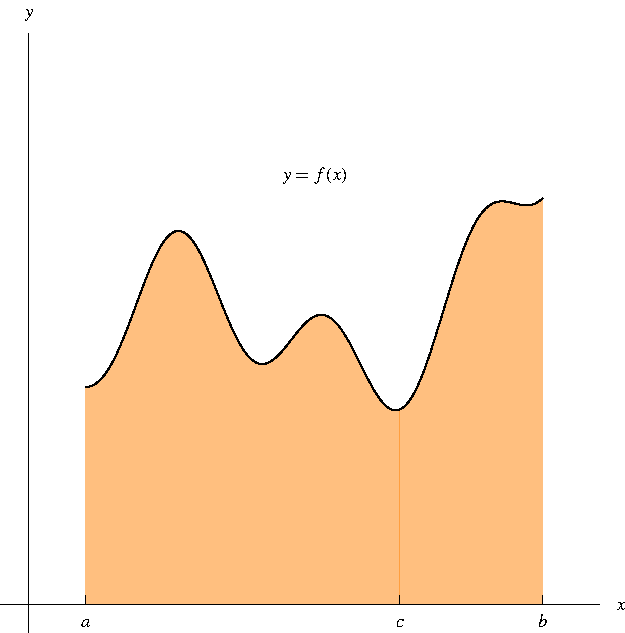
\includegraphics[height=5.6cm]{integration/pictures/05-02-splita.pdf}%
%}%
%\only<handout:0| 2>{%
%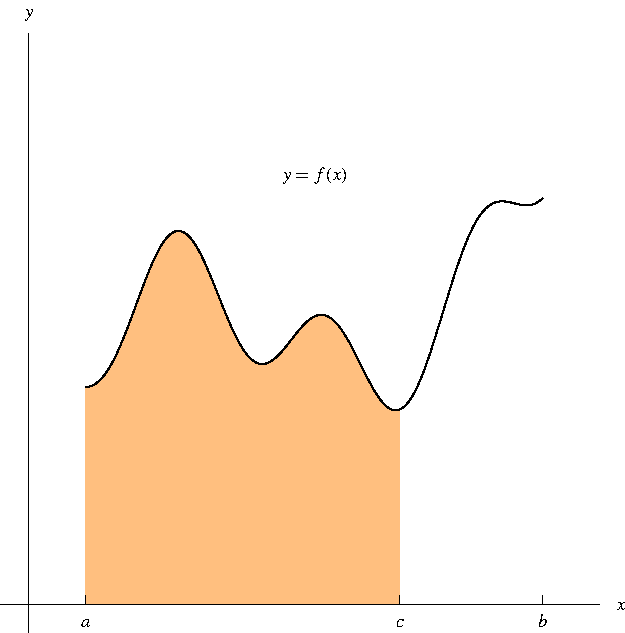
\includegraphics[height=5.6cm]{integration/pictures/05-02-splitb.pdf}%
%}%
%\only<handout:0| 3>{%
%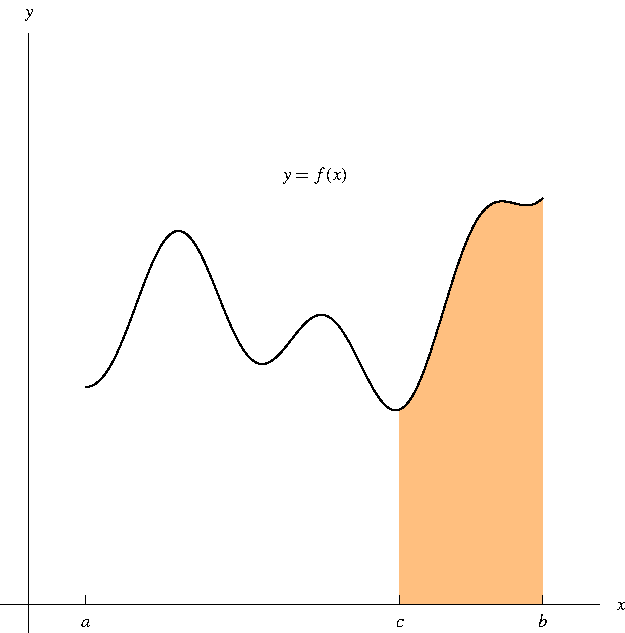
\includegraphics[height=5.6cm]{integration/pictures/05-02-splitc.pdf}%
%}%
\end{center}
\end{frame}
% end module definite-integral-properties-split

%% begin module definite-integral-properties-ex7
\begin{frame}
\begin{example} %[Example 7, p. 352]
If it is known that \alert<handout:0| 5-6>{$\int_0^{10}f(x)\diff x = 17$} and \alert<handout:0| 7-8>{$\int_0^8 f(x) \diff x = 12$}, then find $\int_8^{10}f(x) \diff x$.
\abovedisplayskip=0pt
\belowdisplayskip=0pt
\abovedisplayshortskip=0pt
\belowdisplayshortskip=0pt
\begin{align*}
\uncover<2->{%
\int_{\alert<handout:0| 2-3>{0}}^{\alert<handout:0| 2-3>{8}} f(x)\diff x + \int_{\alert<handout:0| 2-3>{8}}^{\alert<handout:0| 2-3>{10}}f(x)\diff x%
}%
& \uncover<3->{ = } %
\uncover<3->{%
\int_{\alert<handout:0| 3>{0}}^{\alert<handout:0| 3>{10}}f(x)\diff x%
}\\%
\uncover<4->{%
\int_{\alert<handout:0| 2-3>{8}}^{\alert<handout:0| 2-3>{10}}f(x)\diff x%
}%
& \uncover<4->{ = } %
\uncover<4->{%
\alert<handout:0| 5-6>{\int_{\alert<handout:0| 3>{0}}^{\alert<handout:0| 3>{10}}f(x)\diff x} - \alert<handout:0| 7-8>{\int_{\alert<handout:0| 2-3>{0}}^{\alert<handout:0| 2-3>{8}} f(x)\diff x}%
}\\%
& \uncover<5->{ = } %
\uncover<5->{%
\alert<handout:0| 5-6>{\uncover<6->{17}} - \alert<handout:0| 7-8>{\uncover<8->{12}}%
}\\%
& \uncover<9->{ = } %
\uncover<9->{%
5%
}%
\end{align*}
\end{example}
\end{frame}
% end module definite-integral-properties-ex7

% WARNING: This next module could use some pictures.
%% begin module definite-integral-properties-comparison
\begin{frame}[t]
Comparison Properties of the Integral
\begin{enumerate}
\setcounter{enumi}{5}
\item  If $f(x)\geq 0$ for all $a\leq x \leq b$, then $\displaystyle \int_{a}^{b} f(x)\diff x \geq 0$.
\end{enumerate}
\end{frame}

\begin{frame}[t]
Comparison Properties of the Integral
\begin{enumerate}
\setcounter{enumi}{6}
\item  If $f(x)\leq g(x)$ for all $a\leq x \leq b$, then $\displaystyle \int_{a}^{b} f(x)\diff x \leq \int_{a}^{b} g(x)\diff x$.
\end{enumerate}
\begin{center}
\psset{xunit=0.9cm, yunit=0.9cm}
\begin{pspicture}(-0.5,-0.5)(6,4.5)
\psframe*[linecolor=white](-0.5,-0.5)(6,4.5)
\tiny
\rput[l](5.1, 2.6){$y=g(x)$}
\rput[l](5.1, 1.3){$y=f(x)$}
\uncover<2>{
\pscustom*[linecolor=cyan]{
\psplot[linecolor=red, plotpoints=1000]{0.2}{5}{x 2 exp -0.18 mul x 3 exp 0.025 mul x 0.368 mul 0.808 add add add }
\psline(5,0)(0.2,0)
}
}
\uncover<3->{
\pscustom*[linecolor=cyan]{
\psplot[linecolor=red, plotpoints=1000]{0.2}{5}{x -9.9495 mul x 3 exp -2.0625 mul x 4 exp 0.1875 mul x 2 exp 7.4925 mul 5.6936 add add add add }
\psline(5,0)(0.2,0)
}
}
%Function formula: 101/125+46/125 (x)+1/40 ((x)^{3})-9/50 ((x)^{2})
\psplot[linecolor=red, plotpoints=1000]{0.2}{5}{x 2 exp -0.18 mul x 3 exp 0.025 mul x 0.368 mul 0.808 add add add }
%Function formula: 7117/1250+2997/400 ((x)^{2})+3/16 ((x)^{4})-33/16 ((x)^{3})-19899/2000 (x)
\psaxes[ticks=none, labels=none]{<->}(0,0)(-0.5,-0.5)(6,4.5)
\psplot[linecolor=red, plotpoints=1000]{0.2}{5}{x -9.9495 mul x 3 exp -2.0625 mul x 4 exp 0.1875 mul x 2 exp 7.4925 mul 5.6936 add add add add }
\psline(0.2, -0.1)(0.2, 0.1)
\rput[t](0.2, -0.15){$a$}
\psline(5, -0.1)(5, 0.1)
\rput[t](5, -0.15){$b$}
\end{pspicture}
%\only<handout:0| -1>{%
%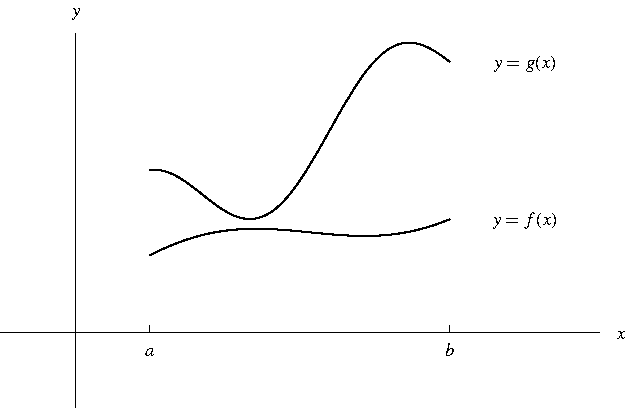
\includegraphics[height=4.2cm]{integration/pictures/05-02-comparisona.pdf}%
%}%
%\only<handout:0| 2>{%
%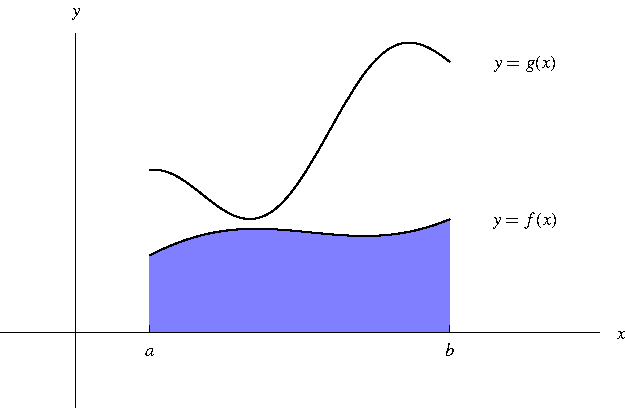
\includegraphics[height=4.2cm]{integration/pictures/05-02-comparisonb.pdf}%
%}%
%\only<handout:0| 3>{%
%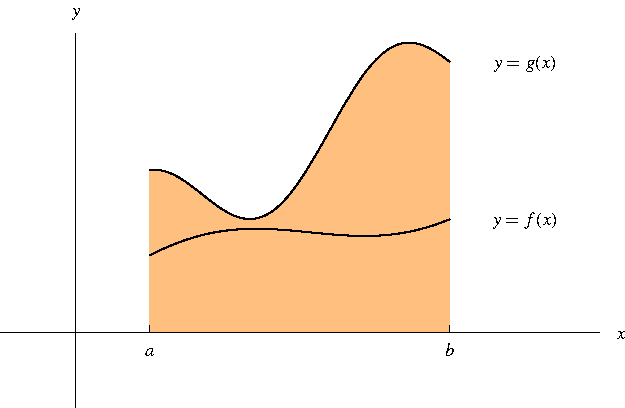
\includegraphics[height=4.2cm]{integration/pictures/05-02-comparisonc.pdf}%
%}%
\[
\alertNoH{ 2}{\int_a^b f(x) \diff x}%
 \leq  %
\alertNoH{ 3}{\int_a^b g(x) \diff x}%
\]
\end{center}
\end{frame}

\begin{frame}[t]
Comparison Properties of the Integral
\begin{enumerate}
\setcounter{enumi}{7}
\item  If $m\leq f(x)\leq M$ for all $a\leq x \leq b$, then
\[
\alertNoH{ 2}{m(b-a)}%
 \leq  %
\alertNoH{ 3}{\int_a^b f(x) \diff x}%
 \leq  %
\alertNoH{ 4}{M(b-a)}%
\]
\end{enumerate}
\begin{center}
\psset{xunit=0.9cm, yunit=0.9cm}
\begin{pspicture}(-0.5,-0.5)(6,4.5)
\psframe*[linecolor=white](-0.5,-0.5)(6,4.5)
\tiny
\uncover<2>{
\pscustom*[linecolor=orange]{
\psplot[linecolor=\fcColorGraph, plotpoints=1000]{0.2}{5}{0.7}
\psline(5,0)(0.2,0)
}
}

\uncover<3>{
\pscustom*[linecolor=cyan!50]{
\psplot[linecolor=\fcColorGraph, plotpoints=1000]{0.2}{5}{x -9.9495 mul x 3 exp -2.0625 mul x 4 exp 0.1875 mul x 2 exp 7.4925 mul 5.6936 add add add add }
\psline(5,0)(0.2,0)
}
}
\uncover<4>{
\pscustom*[linecolor=cyan]{
\psplot[linecolor=red, plotpoints=1000]{0.2}{5}{4.3}
\psline(5,0)(0.2,0)
}
}
%Function formula: 7117/1250+2997/400 ((x)^{2})+3/16 ((x)^{4})-33/16 ((x)^{3})-19899/2000 (x)
\psaxes[ticks=none, labels=none]{<->}(0,0)(-0.5,-0.5)(6,4.5)
\psplot[linecolor=\fcColorGraph, plotpoints=1000]{0.2}{5}{x -9.9495 mul x 3 exp -2.0625 mul x 4 exp 0.1875 mul x 2 exp 7.4925 mul 5.6936 add add add add }
\psline[linecolor=\fcColorGraph](0.2, 0.7)(5,0.7)
\psline[linecolor=\fcColorGraph](0.2, 4.3)(5, 4.3)


\rput[r](4.9, 2.6){\alertNoH{3}{$y=f(x)$}}
\psline[linestyle=dotted, arrows=<->](5.05, 0)(5.05, 0.7)
\rput[l](5.15,0.35){\alertNoH{2}{$m$}}
\psline[linestyle=dotted, arrows=<->](5.5, 0)(5.5, 4.3)
\rput[l](5.6,2.15){\alertNoH{4}{$M$}}

\psline(0.2, -0.1)(0.2, 0.1)
\rput[t](0.2, -0.15){\alertNoH{2,4}{$a$}}
\psline(5, -0.1)(5, 0.1)
\rput[t](5, -0.15){\alertNoH{2,4}{$b$}}
\end{pspicture}
%\only<handout:0| -1>{%
%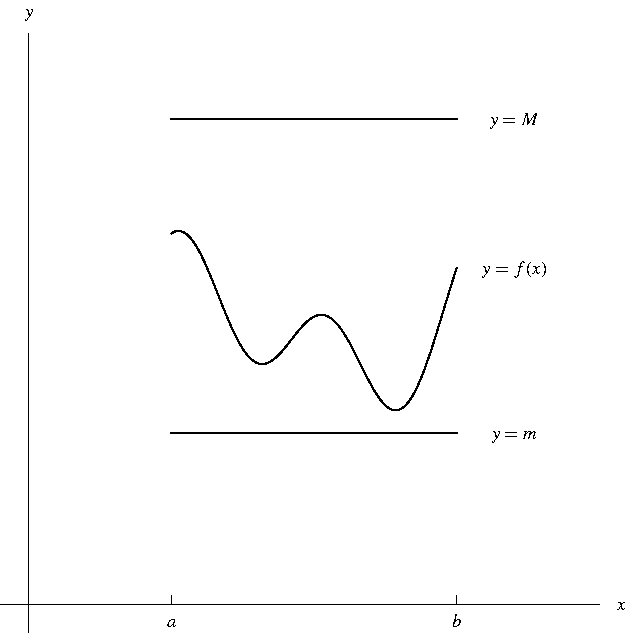
\includegraphics[height=5.6cm]{integration/pictures/05-02-boundinga.pdf}%
%}%
%\only<handout:0| 2>{%
%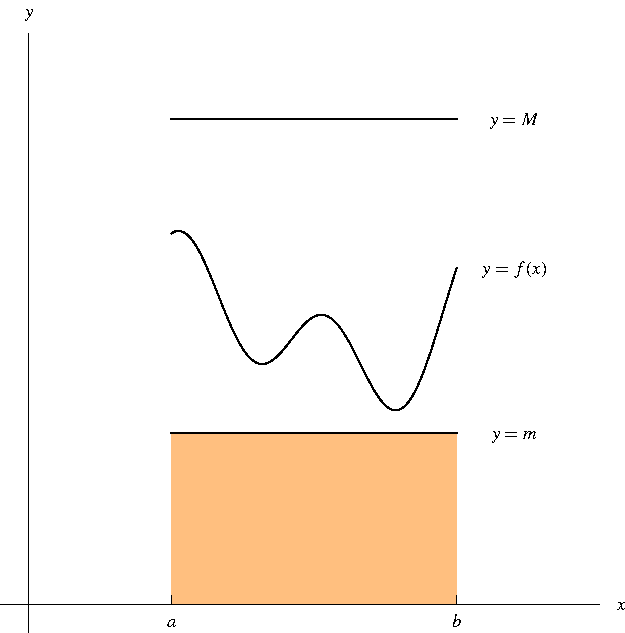
\includegraphics[height=5.6cm]{integration/pictures/05-02-boundingb.pdf}%
%}%
%\only<handout:0| 3>{%
%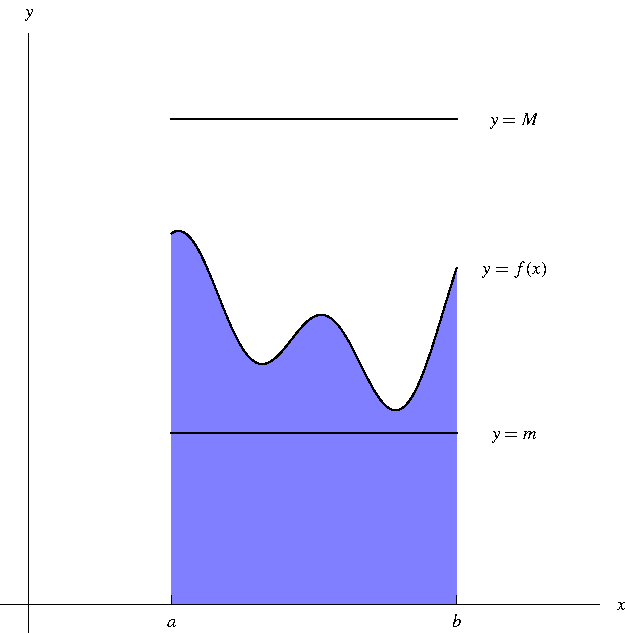
\includegraphics[height=5.6cm]{integration/pictures/05-02-boundingc.pdf}%
%}%
%\only<handout:0| 4>{%
%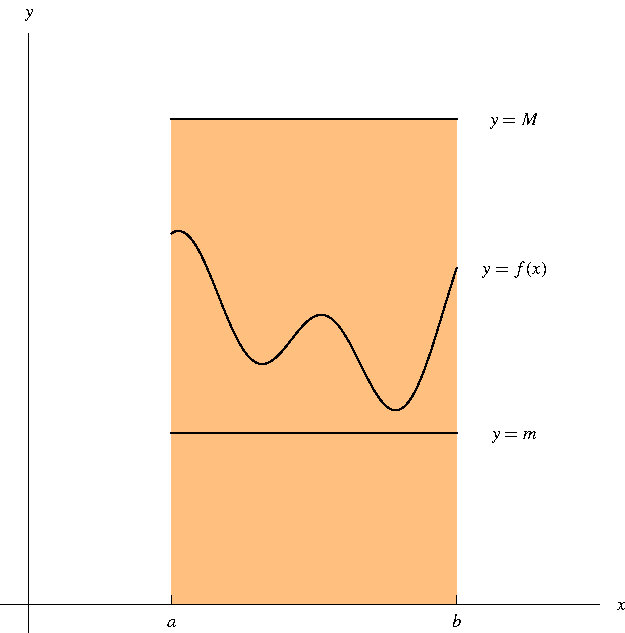
\includegraphics[height=5.6cm]{integration/pictures/05-02-boundingd.pdf}%
%}%
\end{center}
\end{frame}
% end module definite-integral-properties-comparison

%% begin module FTC-part2-ex7
\begin{frame}
\begin{example} %[Example 2, p. 357]
\begin{columns}
\column{0.2\textwidth}
\psset{xunit=0.4cm, yunit=0.4cm}
\begin{pspicture}(-1.000000, -5)(1.500000,5) 
\psframe*[linecolor=white](-1.000000,-5)(7,5) 
\tiny 
\pscustom*[linecolor=cyan]{ %Function formula: \cos{}x 
\psplot[linecolor=\psColorGraph, plotpoints=1000]{0}{1}{x 57.29578 mul cos }\psline(1.000000, 0)(0.000000, 0)}
%Function formula: \cos{}x 
\psplot[linecolor=\psColorGraph, plotpoints=1000]{0}{6}{x 57.29578 mul cos }
\psaxesStandard{-0.6}{-0.6}{6}{1.1}
\end{pspicture} 
\column{0.8\textwidth}
Find the area under the cosine curve from $0$ to $b$, where $0 \leq b \leq \pi /2$.
\begin{itemize}
\item<2->  $\cos x$ is continuous on $[0, \pi /2]$ (in fact, it's continuous everywhere).
\item<3-| alert@3-4>  An antiderivative is \uncover<4->{$\sin x$.}
\end{itemize}
\[
\uncover<5->{%
\int_{\alert<handout:0| 5>{0}}^{\alert<handout:0| 5>{b}} \cos x \ \diff x = \left[ \sin x \right]_{\alert<handout:0| 5>{0}}^{\alert<handout:0| 5>{b}} %
}%
\uncover<6->{%
 = \sin (b) - \sin (0)%
}%
\uncover<7->{%
 = \sin b%
}%
\]
\end{columns}
\end{example}
\end{frame}
% end module FTC-part2-ex7

%% begin module area-def
\begin{frame}
Estimate the area under the curve $y = f(x)$ between $a$ and $b$.
\begin{columns}
\column{.55\textwidth}
\psset{xunit=3cm, yunit=3cm}
\begin{pspicture}(-5, -5)(5,5)
\psframe*[linecolor=white](-5,-5)(5,5)
\psaxes[ticks=none, labels=none]{<->}(0,0)(-0.1,-0.1)(1.7,0.9)
\tiny

\uncover<1>{
\psline*[linecolor=\fcColorAreaUnderGraph, linewidth=0.1pt](0.425, 0)(0.425, 0.339931)(0.3, 0.339931)(0.3, 0)(0.55, 0)(0.55, 0.316508)(0.425, 0.316508)(0.425, 0)(0.675, 0)(0.675, 0.348456)(0.55, 0.348456)(0.55, 0)(0.8, 0)(0.8, 0.416)(0.675, 0.416)(0.675, 0)(0.925, 0)(0.925, 0.499364)(0.8, 0.499364)(0.8, 0)(1.05, 0)(1.05, 0.578773)(0.925, 0.578773)(0.925, 0)(1.175, 0)(1.175, 0.634452)(1.05, 0.634452)(1.05, 0)(1.3, 0)(1.3, 0.646625)(1.175, 0.646625)(1.175, 0)(1.425, 0)(1.425, 0.595517)(1.3, 0.595517)(1.3, 0)(1.55, 0)(1.55, 0.461352)(1.425, 0.461352)(1.425, 0)
\psline[linecolor=blue, linewidth=0.1pt](0.425, 0)(0.425, 0.339931)(0.3, 0.339931)(0.3, 0)(0.55, 0)(0.55, 0.316508)(0.425, 0.316508)(0.425, 0)(0.675, 0)(0.675, 0.348456)(0.55, 0.348456)(0.55, 0)(0.8, 0)(0.8, 0.416)(0.675, 0.416)(0.675, 0)(0.925, 0)(0.925, 0.499364)(0.8, 0.499364)(0.8, 0)(1.05, 0)(1.05, 0.578773)(0.925, 0.578773)(0.925, 0)(1.175, 0)(1.175, 0.634452)(1.05, 0.634452)(1.05, 0)(1.3, 0)(1.3, 0.646625)(1.175, 0.646625)(1.175, 0)(1.425, 0)(1.425, 0.595517)(1.3, 0.595517)(1.3, 0)(1.55, 0)(1.55, 0.461352)(1.425, 0.461352)(1.425, 0)
}
\uncover<2->{
\psline*[linecolor=\fcColorAreaUnderGraph, linewidth=0.1pt](0.3, 0)(0.3, 0.4385)(0.425, 0.4385)(0.425, 0)(0.425, 0)(0.425, 0.339931)(0.55, 0.339931)(0.55, 0)(0.55, 0)(0.55, 0.316508)(0.675, 0.316508)(0.675, 0)(0.675, 0)(0.675, 0.348456)(0.8, 0.348456)(0.8, 0)(0.8, 0)(0.8, 0.416)(0.925, 0.416)(0.925, 0)(0.925, 0)(0.925, 0.499364)(1.05, 0.499364)(1.05, 0)(1.05, 0)(1.05, 0.578773)(1.175, 0.578773)(1.175, 0)(1.175, 0)(1.175, 0.634452)(1.3, 0.634452)(1.3, 0)(1.3, 0)(1.3, 0.646625)(1.425, 0.646625)(1.425, 0)(1.425, 0)(1.425, 0.595517)(1.55, 0.595517)(1.55, 0)
\psline[linecolor=blue, linewidth=0.1pt](0.3, 0)(0.3, 0.4385)(0.425, 0.4385)(0.425, 0)(0.425, 0)(0.425, 0.339931)(0.55, 0.339931)(0.55, 0)(0.55, 0)(0.55, 0.316508)(0.675, 0.316508)(0.675, 0)(0.675, 0)(0.675, 0.348456)(0.8, 0.348456)(0.8, 0)(0.8, 0)(0.8, 0.416)(0.925, 0.416)(0.925, 0)(0.925, 0)(0.925, 0.499364)(1.05, 0.499364)(1.05, 0)(1.05, 0)(1.05, 0.578773)(1.175, 0.578773)(1.175, 0)(1.175, 0)(1.175, 0.634452)(1.3, 0.634452)(1.3, 0)(1.3, 0)(1.3, 0.646625)(1.425, 0.646625)(1.425, 0)(1.425, 0)(1.425, 0.595517)(1.55, 0.595517)(1.55, 0)
}
\rput[t](0.3,-0.03){$a$}
\rput[t](0.425,-0.03){$x_1$}
\rput[t](0.55,-0.03){$x_2$}
%\rput[t](0.675,-0.03){}
%\rput[t](0.8,-0.03){$\frac{4}{5}$}
\rput[t](0.7375,-0.06){$\dots$}
\rput[t](0.925,-0.03){$x_{i-1}$}
\rput[t](1.05,-0.03){$x_{i}$}
%\rput[t](1.175,-0.03){$x_i$}
%\rput[t](1.3,-0.03){$\frac{13}{10}$}
\rput[t](1.3,-0.06){$\dots$}
%\rput[t](1.425,-0.03){$\frac{57}{40}$}
\rput[t](1.55,-0.03){$b$}
%Function formula: -171/50 (x)-27/16 ((x)^{3})+11/10+729/160 ((x)^{2})
\psplot[linecolor=red, plotpoints=1000]{0.3}{1.55}{x 2 exp 4.55625 mul 1.1 add x 3 exp -1.6875 mul add x -3.42 mul add }
\psline{<->}(1.6,0)(1.6, 0.578773)
\psline[linestyle=dotted](1.6, 0.578773)(1.05, 0.578773)
\rput[l](1.6, 0.3343865){$f(x_i)$}
\rput[b](0.9875,0.70773){$\Delta x$}
\psline(0.925,0.668773)(1.05, 0.668773)
\psline(0.925,0.648773)(0.925,0.688773)
\psline(1.05, 0.648773)(1.05, 0.688773)

%\psbrace[linecolor=red,ref=lC](2)(3){Text I}
%\uput{:U}{$\overbrace{}^\text{\normalsize A line}$}
\end{pspicture}
%\only<handout:1| -1>{%
%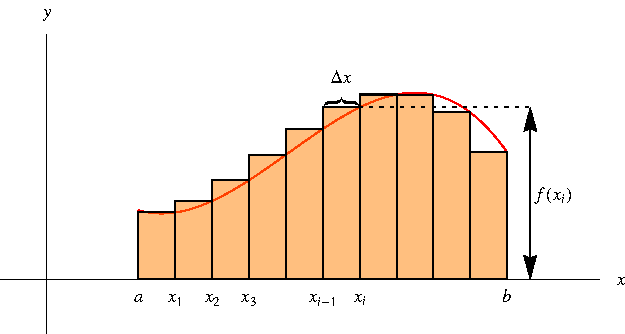
\includegraphics[height=3.5cm]{integration/pictures/05-01-rectangles-right.pdf}%
%}%
%\only<handout:2| 2->{%
%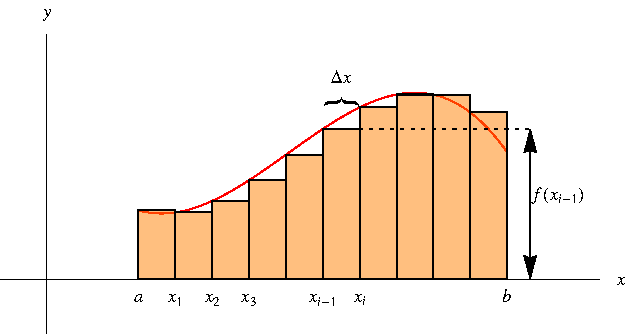
\includegraphics[height=3.5cm]{integration/pictures/05-01-rectangles-left.pdf}%
%}%



\begin{itemize}
\item<1->  The width of the interval is $b-a$.
\item<1->  The width of each of the $n$ strips is $\Delta x = \frac{b-a}{n}$.
\item<1->  The strips divide $[a,b]$ into $n$ subintervals:\\ $[x_0, x_1]$, $[x_1,x_2]$, $\ldots ,$ $[x_{n-1},x_n]$,\\ where $x_0 = a$ and $x_n = b$.
\end{itemize}
\column{.45\textwidth}
\begin{itemize}
\item<1->  The \only<handout:1| -1>{right}\only<handout:2| 2->{\alert<handout:2| 2>{left}} endpoints of the subintervals are
\end{itemize}
\abovedisplayskip=0pt
\belowdisplayskip=0pt
\begin{eqnarray*}
x_{\only<handout:1| -1>{1}\only<handout:2| 2->{\alert<handout:2| 2>{0}}} & = & a \only<handout:1| -1>{+ \Delta x}\\
x_{\only<handout:1| -1>{2}\only<handout:2| 2->{\alert<handout:2| 2>{1}}} & = & a + \only<handout:1| -1>{2}\Delta x\\
x_{\only<handout:1| -1>{3}\only<handout:2| 2->{\alert<handout:2| 2>{2}}} & = & a + \only<handout:1| -1>{3}\only<handout:2| 2->{2}\Delta x\\
& \vdots &
\end{eqnarray*}
\begin{itemize}
\item<1->  The height of the $i$th rectangle is $f(x_{i\only<handout:2| 2->{\alert<handout:2| 2>{-1}}})$.
\item<1->  The area of the $i$th rectangle is $f(x_{i\only<handout:2| 2->{\alert<handout:2| 2>{-1}}})\Delta x$.
\end{itemize}
\end{columns}
\abovedisplayskip=0pt
\belowdisplayskip=0pt
\[
\only<handout:1| -1>{R_n}\only<handout:2| 2->{\alert<handout:2| 2>{L_n}} = f(x_{\only<handout:1| -1>{1}\only<handout:2| 2->{\alert<handout:2| 2>{0}}})\Delta x + f(x_{\only<handout:1| -1>{2}\only<handout:2| 2->{\alert<handout:2| 2>{1}}})\Delta x + f(x_{\only<handout:1| -1>{3}\only<handout:2| 2->{\alert<handout:2| 2>{2}}})\Delta x + \cdots + f(x_{n\only<handout:2| 2->{\alert<handout:2| 2>{-1}}})\Delta x
\]
\end{frame}

\begin{frame}
\begin{definition}[Area Under a Curve]
The area of the region $S$ that lies under the curve $y = f(x)$ is the limit of the sum of the areas of the approximating rectangles:
\abovedisplayskip=0pt
\belowdisplayskip=0pt
\[
A = \lim_{n\to\infty} R_n = \lim_{n\to\infty} [ f(x_1)\Delta x + f(x_2) \Delta x + \cdots + f(x_n) \Delta x]
\]
\end{definition}
\begin{itemize}
\item<2->  This limit always exists if $f$ is continuous.
\item<3->  If $f$ is continuous, we get the same limit if we use left endpoints:
\abovedisplayskip=0pt
\belowdisplayskip=0pt
\[
A = \lim_{n\to\infty} L_n = \lim_{n\to\infty} [ f(x_0)\Delta x + f(x_1) \Delta x + \cdots + f(x_{n-1}) \Delta x]
\]
\item<4->  If $f$ is continuous, we get the same limit if we use any number $x_i^*$ in the interval $[x_{i-1},x_i]$.  $x_i^*$ is called a sample point.
\abovedisplayskip=0pt
\belowdisplayskip=0pt
\[
A = \lim_{n\to\infty} [ f(x_1^*)\Delta x + f(x_2^*) \Delta x + \cdots + f(x_{n}^*) \Delta x]
\]
\end{itemize}
\uncover<5->{%
\begin{definition}[Riemann Sum]
A Riemann sum is any sum of the form
\abovedisplayskip=0pt
\belowdisplayskip=0pt
\[
f(x_1^*)\Delta x + f(x_2^*) \Delta x + \cdots + f(x_{n}^*) \Delta x.
\]
\end{definition}
}%
\end{frame}
% end module area-def

%% begin module definite-integral-def
\begin{frame}\frametitle{ %(5.2) 
The Definite Integral}
\begin{definition}[Definite Integral]
\begin{itemize}
\item  Let $f$ be a function defined for $a\leq x\leq b$.
\item  Divide the interval $[a,b]$ into $n$ subintervals of equal width $\Delta x = (b-a)/n$ nd set $x_0=a$, $x_n=b$.
\item  Let $x_0$, $x_1,\ldots ,$ $x_n $ be the endpoints of the subintervals.
\item  Let $x_1^*, x_2^*, \ldots , x_n^*$ be any sample points in these subintervals; that is, $x_i^*$ is in $[x_{i-1},x_i]$.  
\end{itemize}
\abovedisplayskip=0pt
\belowdisplayskip=0pt
Suppose the limit $\lim\limits_{n\to \infty} \sum\limits_{i=1}^n f(x_i^*)\Delta x$ exists and is independent of the choice of sample points $x_i^*$. Then we call this limit the integral of $f$ over $[a,b]$ and write
\[
\int_a^b f(x) \diff x = \lim_{n\to \infty} \sum_{i=1}^n f(x_i^*)\Delta x \quad .
\]
\end{definition}
\end{frame}

\begin{frame}
\[
\mathop{\alert<handout:0| 2>{\int}}_{\alert<handout:0| 4>{a}}^{\alert<handout:0| 4>{b}} \alert<handout:0| 3>{f(x)} \alert<handout:0| 0>{\diff x} = \lim_{n\to \infty} \sum_{i=1}^n f(x_i^*)\Delta x,
\]
\begin{itemize}
\item<1-| alert@2>  $\int$ is called the integration sign.
\item<1-| alert@3>  $f(x)$ is called the integrand.
\item<1-| alert@4>  $a$ and $b$ are called the limits of integration.
\item<5->  The definite integral is a number.  It does not depend on $x$.  We could use any variable instead of $x$.
\end{itemize}
\uncover<5->{%
\[
\int_a^b f(x) \diff x = \int_a^b f(t)\diff t = \int_a^b f(r)\diff r = \int_a^b f(\theta )\diff \theta
\]
}%
\end{frame}
% end module definite-integral-def

%% begin module FTC-part2
\begin{frame}
\uncover<3->{
\begin{theorem}
Let $f$ be a continuous function on $[a,b]$. Then $f$ is integrable over $[a,b]$.
\end{theorem}
}
\uncover<2->{
\uncover<3->{In other words,} \alert<2>{$\displaystyle\int_a^{b}f(x)dx $ is defined for any continuous (over $[a,b]$) function $f$}.
}

\begin{theorem}[The Evaluation Theorem (FTC part 2)]
If \alert<2>{$f$ is continuous on $[a, b]$}, then
\[
\alert<2>{\int_a^b f(x) \diff x} = F(b) - F(a),
\]
where $F$ is any antiderivative of $f$.
\end{theorem}

\end{frame}
% end module FTC-part2


%% begin module definite-integral-def
\begin{frame}\frametitle{ %(5.2) 
The Definite Integral}
\begin{definition}[Definite Integral]
\begin{itemize}
\item  Let $f$ be a function defined for $a\leq x\leq b$.
\item  Divide the interval $[a,b]$ into $n$ subintervals of equal width $\Delta x = (b-a)/n$ nd set $x_0=a$, $x_n=b$.
\item  Let $x_0$, $x_1,\ldots ,$ $x_n $ be the endpoints of the subintervals.
\item  Let $x_1^*, x_2^*, \ldots , x_n^*$ be any sample points in these subintervals; that is, $x_i^*$ is in $[x_{i-1},x_i]$.  
\end{itemize}
\abovedisplayskip=0pt
\belowdisplayskip=0pt
Suppose the limit $\lim\limits_{n\to \infty} \sum\limits_{i=1}^n f(x_i^*)\Delta x$ exists and is independent of the choice of sample points $x_i^*$. Then we call this limit the integral of $f$ over $[a,b]$ and write
\[
\int_a^b f(x) \diff x = \lim_{n\to \infty} \sum_{i=1}^n f(x_i^*)\Delta x \quad .
\]
\end{definition}
\end{frame}

\begin{frame}
\[
\mathop{\alert<handout:0| 2>{\int}}_{\alert<handout:0| 4>{a}}^{\alert<handout:0| 4>{b}} \alert<handout:0| 3>{f(x)} \alert<handout:0| 0>{\diff x} = \lim_{n\to \infty} \sum_{i=1}^n f(x_i^*)\Delta x,
\]
\begin{itemize}
\item<1-| alert@2>  $\int$ is called the integration sign.
\item<1-| alert@3>  $f(x)$ is called the integrand.
\item<1-| alert@4>  $a$ and $b$ are called the limits of integration.
\item<5->  The definite integral is a number.  It does not depend on $x$.  We could use any variable instead of $x$.
\end{itemize}
\uncover<5->{%
\[
\int_a^b f(x) \diff x = \int_a^b f(t)\diff t = \int_a^b f(r)\diff r = \int_a^b f(\theta )\diff \theta
\]
}%
\end{frame}
% end module definite-integral-def

%% begin module continuous-functions-integrable
\begin{frame}
\begin{theorem}
Let $f$ be a continuous function on $[a,b]$. Then $f$ is integrable over $[a,b]$.
\end{theorem}
\begin{itemize}
\item In particular the integral does not depend the choice of sampling points so long as the intervals containing them shrink.
\item The proof of this theorem is not difficult, but is outside of the scope of Calculus I and II.
\item The only ``difficulty'' in the proof stems from the fact that we have not rigorously constructed the real numbers. 
\item We already (silently) assumed a construction of the real numbers when we defined limits. 
\item Such a construction is also (silently) assumed in most regular high school mathematics courses.
%\item  The proof of the Theorem uses the fact that every set bounded above has a least upper bound. The latter fact is either taken as an axiom of the real numbers, or is proven from equivalent set of axioms. This is the main fact a calculus student is missing to understand/prove on one's own the above theorem.
\item A student interested in a proof of the theorem should google ``Darboux integral''.
\end{itemize}

\end{frame}
% end module continuous-functions-integrable

%%module FTC part1 solving problems.
\begin{frame}
\begin{theorem}
Let $A,B$-numbers, $a(x), b(x)$ -differentiable functions with $A<a(x)<B$, $A<b(x)<B$. Let $f$ - continuous on $[A,B]$  and $\displaystyle G(x)=\int_{a(x)}^{b(x)} f(t)dt$. Then  $ \alertNoH{11}{G'(x)=f(b(x))b'(x)-f(a(x))a'(x)}$.
\end{theorem}
\begin{proof}
\uncover<2->{\alertNoH{6}{Let $c\in (A, B)$}.} \uncover<3->{Set $\alertNoH{7}{\displaystyle h(u)=\int_{c}^{u}f(t)dt}$.} \uncover<4->{FTC part 1 states that $h'(u)=f(u)$.}

$\begin{array}{rcl}
\uncover<5->{\displaystyle G(x)&=&\displaystyle\int_{a(x)}^{b(x)} f(t)dt}\uncover<6->{= \int_{\alertNoH{6}{c}}^{b(x)} f(t)dt+ \int_{\alertNoH{7}{a(x)}}^{\alertNoH{6}{\alertNoH{7}{c}}} f(t)dt} \\
\uncover<7->{&=&\displaystyle \int_c^{b(x)} f(t)dt\alertNoH{7}{-}\int_{\alertNoH{7}{c}}^{\alertNoH{7}{a(x)}}f(t)dt}\uncover<8->{=\alertNoH{8}{h(b(x))-h(a(x)) } \quad.}
\end{array}$

\uncover<9->{Then} \uncover<10->{using the chain rule we get}

$ \uncover<9->{\displaystyle\alertNoH{11}{  G'(x)}= \left(h(b(x))-h(a(x)) \right)'} \uncover<10->{= h'(b(x)) b'(x)-h'(a(x))a'(x)}\uncover<11->{=\alertNoH{11}{f(b(x))b'(x)-f(a(x))a'(x)},}
$\uncover<11->{ as desired.}
\end{proof}
\end{frame}

\begin{frame}
Problems similar to the following often appear on Calculus I exams.
\begin{example}
Let $\displaystyle G(x)=\int_{\sqrt{x}}^{x^2}\ln t dt$, $x> 0$. Find $G'(x)$.

\[
\uncover<2->{G'(x)=(\ln x^2) (x^2)'-(\ln \sqrt{x}) (\sqrt{x})'}\uncover<3->{= \left(4x- \frac14 x^{-\frac12}\right)\ln x.}
\]

\end{example}
\end{frame}

%end module FTC part1 solving problems.


%% begin module FTC1-proof
\begin{frame}
\begin{theorem}[The Fundamental Theorem of Calculus part 1]
Let \alertNoH{2}{$f$ be a function continuous on $[a, b]$} and let $G(x) = \displaystyle \int_a^x f(t) \diff t$ for all $x\in [a,b]$. Then $G$ is differentiable and $G'(x) = f(x)$.
\end{theorem}
\begin{proof}[Proof]
\begin{columns}
\column{0.27\textwidth}
\psset{xunit=0.9cm, yunit=0.9cm}

\begin{pspicture}(-0.6,-0.6)(3.3,3.3)
\psframe*[linecolor=white](-0.6,-0.6)(3.3,3.3)
\tiny
%\fcLabels{3}{2.5}

\pscustom*[linecolor=cyan]{
\psplot[linecolor=\fcColorGraph, plotpoints=1000]{0.5}{2}{1 -0.5 x add 3 exp 0.333333 mul add -0.5 x add 2 exp -0.5 mul add }
\psline(2,0)(0.5,0)
}
\uncover<20,21>{
\pscustom*[linecolor=red]{
\psplot[linecolor=\fcColorGraph, plotpoints=1000]{0.5}{2}{1 -0.5 x add 3 exp 0.333333 mul add -0.5 x add 2 exp -0.5 mul add }
\psline(2,0)(0.5,0)
}
}

\uncover<11->{
\pscustom*[linecolor=blue]{
\psplot[linecolor=\fcColorGraph, plotpoints=1000]{2}{2.15}{1 -0.5 x add 3 exp 0.333333 mul add -0.5 x add 2 exp -0.5 mul add }
\psline(2.15,1.136125)(2.15,0)(2,0)
}
}

\uncover<10,20,22>{
\pscustom*[linecolor=red]{
\psplot[linecolor=\fcColorGraph, plotpoints=1000]{2}{2.15}{1 -0.5 x add 3 exp 0.333333 mul add -0.5 x add 2 exp -0.5 mul add }
\psline(2.15,1.136125)(2.15,0)(2,0)
}
}

\uncover<12>{
\pscustom*[linecolor=red]{
\psplot[linecolor=\fcColorGraph, plotpoints=1000]{2}{2.15}{1 -0.5 x add 3 exp 0.333333 mul add -0.5 x add 2 exp -0.5 mul add }
\psline(2.15,1.136125)(2.15,1)(2,1)
}
}

\psaxes[ticks=none, labels=none]{<->}(0,0)(-0.5,-0.5)(3.2,3.083333)

%Function formula: -1/2 (x-1/2)^{2}+1/3 (x-1/2)^{3}+1
\psplot[linecolor=\fcColorGraph, plotpoints=1000]{0.5}{3}{1 -0.5 x add 3 exp 0.333333 mul add -0.5 x add 2 exp -0.5 mul add }
\rput[b](2.3, 2.4){$y=f(x)$}
\uncover<11,14>{
\psline*[linecolor=red](2,0)(2.15,0)(2.15,1)(2,1)(2,0)
}
\uncover<13->{
\psline(2,0)(2.15,0)(2.15,1.136125)(2,1.136125)(2,0)
}

\fcXTick{2}

\uncover<3>{ %
\psline[linecolor=red, linewidth=2pt](1.5,0)( 2.5,0 )
}
\uncover<4-7>{ %
\psline[linewidth=2pt](1.5,0)( 2.5,0 )
}

\uncover<4>{ %
\psline[linecolor=red, linewidth=2pt](2,0)(2,1)
}

\uncover<6>{ %
\psline(2.4,1.481333)(2.4,0)
}
\uncover<5>{ %
\psline[linecolor=red, linewidth=2pt](2.4,0)(2.4,1.481333)
}

\uncover<5-7>{ %
\psline(2,0)(2,1)
}
\uncover<5>{ %
\psline[linecolor=red](2.4,0)(2.4,1.481333)
}
\uncover<6>{ %
\psline[linecolor=red, linewidth=2pt](2,1)(2, 1.481333)
}
\fcXTickWithLabel{0.5}{$a$}

\fcXTick{3}
\rput[tl](3,-0.2){$b$}
\uncover<7->{
\fcXTick{2.15}
\rput[tl](2.15, -0.2){$x+h$}
}
\uncover<7,13>{
\psline[linecolor=red, linewidth=2pt](2,0)(2.15,0)
}
\rput[tr](2, -0.235){$x$}
\end{pspicture}

\vspace{1.68cm}
\column{0.73\textwidth}

\only<1-15>{
\uncover<2->{\alertNoH{2}{Let $\varepsilon >0$. There \alertNoH{3}{exists $\delta$} such that $\alertNoH{8}{\alertNoH{6}{|\alertNoH{5}{f(t)}-\alertNoH{4}{f(x)}|} < \varepsilon}$ for all $t$ for which $|x-t|<\delta$}.} \uncover<3->{\alertNoH{7}{Then for all $0<h<\delta$:} }
\[
\begin{array}{rlll|l}
\uncover<8->{\alertNoH{8}{\varepsilon} &\alertNoH{8}{ > \hphantom{ \int_{ x}^{ x+h}(} f(t)-f(x) } & \alertNoH{8}{ > - \varepsilon }  &\uncover<9->{&\text{integrate}} }\\
\uncover<9->{h\varepsilon  & >\alertNoH{12}{ \alertNoH{10,11}{\int_{x }^{x+h}} ( \alertNoH{10}{ f(t)}-\alertNoH{11}{f(x)})\alertNoH{10,11}{ dt} }&>-h\varepsilon &\uncover<13->{& \text{divide~by~}\alertNoH{13}{h }} } \\
\uncover<13->{\varepsilon& >\frac{\alertNoH{14}{\int_{x }^{x+h}}(f(t) -\alertNoH{14}{f(x)}) \alertNoH{14}{dt}}{ \alertNoH{13,14}{ h} }& >-\varepsilon}\\
\uncover<14->{\alertNoH{15}{\varepsilon}&\alertNoH{15}{>} \frac{\int_{x }^{x+h}f(t)dt }{h}- \alertNoH{14}{\frac{h f(x)}{h}} &\alertNoH{15}{ > - \varepsilon}}\\
\uncover<15->{\varepsilon&\color{red} >  \left| \color{black} \frac{\int_{x }^{x+h}f(t)dt }{h} - f(x)\color{red} \right|}\\
\end{array}
\]
}

\only<16->{
\uncover<17->{In analogous fashion  \alertNoH{17}{we can handle the case $h<0$}, to prove:} \alertNoH{23}{ for any $\varepsilon >0$ there exists $\delta>0$ so that for \\ all $\only<16>{0<h\phantom{|}} \alertNoH{17}{\only<17->{\phantom{0<}|h|}} \alertNoH{17}{<\delta}$ we have $\left| \frac{\int_{x }^{x+h}f(t)dt }{h}-f(x)\right|<\varepsilon$.}

\[
\begin{array}{l}
\uncover<18->{\displaystyle G'(x)=\lim\limits_{h\to 0}\frac{ \alertNoH{20}{ G(x+h)} -\alertNoH{21}{G(x)}}{h} }\\
\uncover<19->{\displaystyle \phantom{ G'(x) }= \lim\limits_{h\to 0}  \frac{ \alertNoH{20}{ \alertNoH{22}{\int_{a}^{x+h}} f(t)dt} - \alertNoH{21}{ \alertNoH{22}{\int_{a}^{x}} f(t)dt}}{h} }\\
\uncover<22->{\displaystyle \phantom{ G'(x) }= \alertNoH{23}{\lim\limits_{h\to 0}\frac{\alertNoH{22}{\int_{x}^{x+h}}f(t)dt }{h} \uncover<23->{=f(x)}}}
\end{array}
\]

}
\end{columns}
\end{proof}
\end{frame}
% end module FTC1-proof

% begin module limit-ex1
\begin{frame}
\begin{example}[Example 1, p. 96]
\begin{columns}[c]
\column{.5\textwidth}
\uncover<6->{
\ 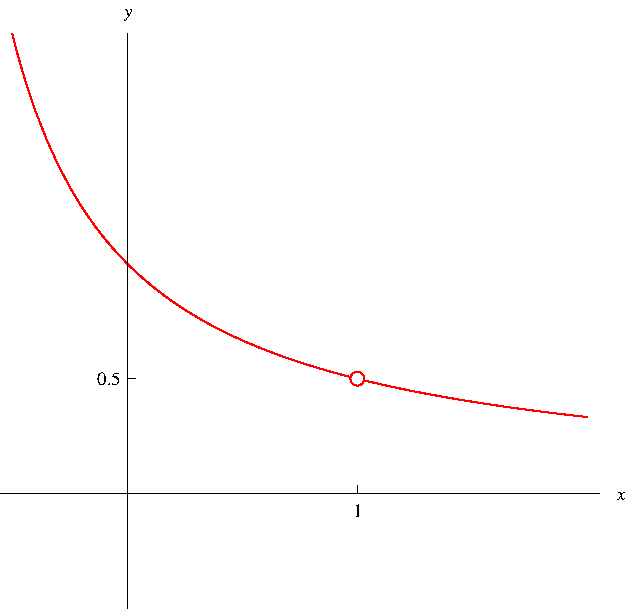
\includegraphics[height=4.5cm]{limits/pictures/02-01-ex1.pdf}%
}
\column{.5\textwidth}
\begin{itemize}
\item  Guess the value of $\lim_{x\rightarrow 1}\frac{x - 1}{x^2 - 1}$.
\item<2->  Notice that $\frac{x-1}{x^2-1}$ doesn't exist at $1$.  
\item<3->  It does exist at values near $1$.
\item<5->  We guess that the limit is $0.5$. 
\item<6->  In this case, our guess is correct.
\end{itemize}
\end{columns}
\uncover<4->{
\[
\begin{array}{|r@{.}l|r@{.}l||r@{.}l|r@{.}l|}
\hline
\multicolumn{2}{|c|}{x} &
\multicolumn{2}{|c||}{f(x)} &
\multicolumn{2}{|c|}{x} &
\multicolumn{2}{|c|}{f(x)} \\
\hline
0 & 
5 & 
0 & 
666667 & 
1 & 
5 & 
0 & 
400000 \\ 
0 & 
9 & 
0 & 
526316 & 
1 & 
1 & 
0 & 
476190 \\ 
0 & 
99 & 
0 & 
502513 & 
1 & 
01 & 
0 & 
497512 \\ 
0 & 
999 & 
0 & 
500250 & 
1 & 
001 & 
0 & 
499750 \\ 
0 & 
9999 & 
0 & 
500025 & 
1 & 
0001 & 
0 & 
499975 \\ 
\hline
\end{array}
\]
}
\end{example}
\end{frame}
% end module limit-ex1

% begin module limit-ex3
\begin{frame}
\begin{example} %[Example 3, p. 98]
\begin{columns}[c]
\column{.5\textwidth}
\uncover<6->{
\psset{xunit=1.5cm,yunit=1.5cm}
\begin{pspicture}(-2,-0.5)(2.2,1.5)
\psframe*[linecolor=white](-2, -0.5)(2.2, 1.7)
\tiny
\fcAxesStandard{-2}{-0.5}{2}{1.5}
\rput[br](-0.1,1.1){ $1$}
\psplot[linecolor=red]{-2}{2}{ x 57.295779513 mul sin x div}
\fcHollowDot{0}{1}
\end{pspicture}
%\ 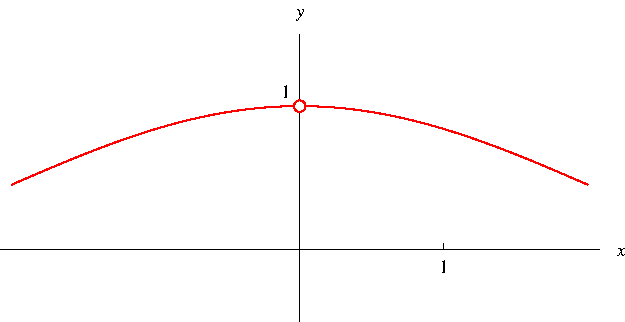
\includegraphics[height=3cm]{limits/pictures/02-01-ex3.pdf}%
}
\column{.5\textwidth}
\begin{itemize}
\item  Guess the value of $\lim_{x\rightarrow 0}\frac{\sin x}{x}$.
\item<2->  Notice that $\frac{\sin x}{x}$ is not defined at $0$.
\item<3->  It is defined for all other values of $x$ near $0$.
\item<5->  We guess that the limit is $1$.
\item<6->  In this case, our guess is correct.
\end{itemize}
\end{columns}
\uncover<4->{
\[
\begin{array}{|r@{.}l|r@{.}l||r@{.}l|r@{.}l|}
\hline
\multicolumn{2}{|c|}{x} &
\multicolumn{2}{|c||}{f(x)} &
\multicolumn{2}{|c|}{x} &
\multicolumn{2}{|c|}{f(x)} \\
\hline
\pm 1 &
0 &
0 &
841471 &
\pm 0 &
1 &
0 &
998334 \\
\pm 0 &
5 &
0 &
958851 &
\pm 0 &
05 &
0 &
999583 \\
\pm 0 &
4 &
0 &
973546 &
\pm 0 &
01 &
0 &
999983 \\
\pm 0 &
3 &
0 &
985067 &
\pm 0 &
005 &
0 &
999995 \\
\pm 0 &
2 &
0 &
993347 &
\pm 0 &
001 &
0 &
999999 \\
\hline
\end{array}
\]
}
\end{example}
\end{frame}
% end module limit-ex3

% begin module limit-ex4
\begin{frame}
\begin{example} %[Example 4, p. 98]
\begin{columns}[c]
\column{.4\textwidth}
\begin{itemize}
\item  Guess the value of $\lim_{x\rightarrow 0}\sin\frac{\pi}{x}$.
\item<2->  Notice that $\sin\frac{\pi}{x}$ doesn't exist at $0$.  
\item<3->  It does exist at values near $0$.
\item<5->  We guess that the limit is $0$. 
\item<6->  In this case, our guess is \alert<6>{wrong}.
\end{itemize}
\column{.6\textwidth}
\uncover<4->{
\[
\begin{array}{|r|c|r|c|}
\hline
x & f(x) & x & f(x) \\
\hline
1 & \sin \pi = 0 &
\frac{1}{2} & \sin 2\pi = 0 \\
\frac{1}{3} & \sin 3\pi = 0 &
\frac{1}{4} & \sin 4\pi = 0 \\
0.1 & \sin 10\pi = 0 &
0.01 & \sin 100\pi = 0 \\
\hline
\end{array}
\]
}

\uncover<6->{
\psset{xunit=1.1cm,yunit=1.1cm}
\begin{pspicture}(-3,-1.5)(3,1.5)
\psframe*[linecolor=white](-3, -1.5)(3.2, 1.7)
\psaxes[ticks=x, labels=none]{<->}(0,0)(-3,-1.5)(3,1.5)
\rput[b](0, 1.52){\tiny $y$}
\rput[l](3.02, 0){\tiny $x$}
\rput[t](1,-0.1){ $1$}
\psplot[linewidth=0.3pt, linecolor=red, plotpoints=10000]{-3}{-0.01}{3.14159 x div 57.295779513 mul sin}
\psplot[linewidth=0.3pt, linecolor=red, plotpoints=10000]{0.01}{3}{3.14159 x div 57.295779513 mul sin}
%\pscircle*[fillcolor=white, linecolor=red](0, 1){0.07}
%\pscircle*[fillcolor=white, linecolor=white](0, 1){0.04}

\end{pspicture}
%\ 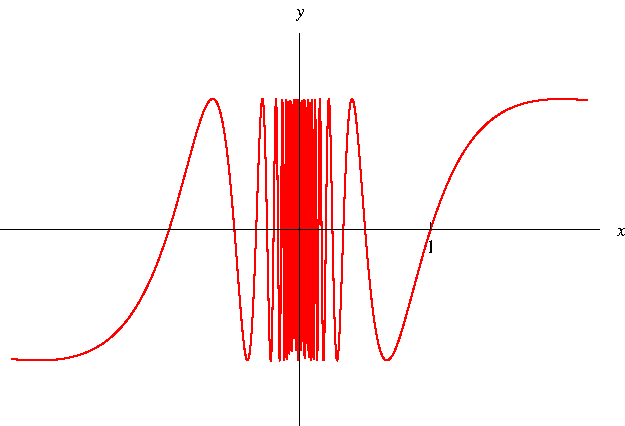
\includegraphics[height=4cm]{limits/pictures/02-01-ex4.pdf}%
}
\end{columns}
\end{example}
\end{frame}
% end module limit-ex4

\end{document}
